% Options for packages loaded elsewhere
\PassOptionsToPackage{unicode}{hyperref}
\PassOptionsToPackage{hyphens}{url}
\PassOptionsToPackage{dvipsnames,svgnames,x11names}{xcolor}
%
\documentclass[
  12pt,
  a4paper,
]{article}
\usepackage{amsmath,amssymb}
\usepackage[]{mathpazo}
\usepackage{setspace}
\usepackage{iftex}
\ifPDFTeX
  \usepackage[T1]{fontenc}
  \usepackage[utf8]{inputenc}
  \usepackage{textcomp} % provide euro and other symbols
\else % if luatex or xetex
  \usepackage{unicode-math}
  \defaultfontfeatures{Scale=MatchLowercase}
  \defaultfontfeatures[\rmfamily]{Ligatures=TeX,Scale=1}
\fi
% Use upquote if available, for straight quotes in verbatim environments
\IfFileExists{upquote.sty}{\usepackage{upquote}}{}
\IfFileExists{microtype.sty}{% use microtype if available
  \usepackage[]{microtype}
  \UseMicrotypeSet[protrusion]{basicmath} % disable protrusion for tt fonts
}{}
\makeatletter
\@ifundefined{KOMAClassName}{% if non-KOMA class
  \IfFileExists{parskip.sty}{%
    \usepackage{parskip}
  }{% else
    \setlength{\parindent}{0pt}
    \setlength{\parskip}{6pt plus 2pt minus 1pt}}
}{% if KOMA class
  \KOMAoptions{parskip=half}}
\makeatother
\usepackage{xcolor}
\usepackage[margin=1in]{geometry}
\usepackage{longtable,booktabs,array}
\usepackage{calc} % for calculating minipage widths
% Correct order of tables after \paragraph or \subparagraph
\usepackage{etoolbox}
\makeatletter
\patchcmd\longtable{\par}{\if@noskipsec\mbox{}\fi\par}{}{}
\makeatother
% Allow footnotes in longtable head/foot
\IfFileExists{footnotehyper.sty}{\usepackage{footnotehyper}}{\usepackage{footnote}}
\makesavenoteenv{longtable}
\usepackage{graphicx}
\makeatletter
\def\maxwidth{\ifdim\Gin@nat@width>\linewidth\linewidth\else\Gin@nat@width\fi}
\def\maxheight{\ifdim\Gin@nat@height>\textheight\textheight\else\Gin@nat@height\fi}
\makeatother
% Scale images if necessary, so that they will not overflow the page
% margins by default, and it is still possible to overwrite the defaults
% using explicit options in \includegraphics[width, height, ...]{}
\setkeys{Gin}{width=\maxwidth,height=\maxheight,keepaspectratio}
% Set default figure placement to htbp
\makeatletter
\def\fps@figure{htbp}
\makeatother
\setlength{\emergencystretch}{3em} % prevent overfull lines
\providecommand{\tightlist}{%
  \setlength{\itemsep}{0pt}\setlength{\parskip}{0pt}}
\setcounter{secnumdepth}{-\maxdimen} % remove section numbering
\pagestyle{plain}
\newlength{\cslhangindent}
\setlength{\cslhangindent}{1.5em}
\newlength{\csllabelwidth}
\setlength{\csllabelwidth}{3em}
\newlength{\cslentryspacingunit} % times entry-spacing
\setlength{\cslentryspacingunit}{\parskip}
\newenvironment{CSLReferences}[2] % #1 hanging-ident, #2 entry spacing
 {% don't indent paragraphs
  \setlength{\parindent}{0pt}
  % turn on hanging indent if param 1 is 1
  \ifodd #1
  \let\oldpar\par
  \def\par{\hangindent=\cslhangindent\oldpar}
  \fi
  % set entry spacing
  \setlength{\parskip}{#2\cslentryspacingunit}
 }%
 {}
\usepackage{calc}
\newcommand{\CSLBlock}[1]{#1\hfill\break}
\newcommand{\CSLLeftMargin}[1]{\parbox[t]{\csllabelwidth}{#1}}
\newcommand{\CSLRightInline}[1]{\parbox[t]{\linewidth - \csllabelwidth}{#1}\break}
\newcommand{\CSLIndent}[1]{\hspace{\cslhangindent}#1}
\usepackage{lineno} % add 
\linenumbers % turns line numbering on 

% Allowing for landscape pages
\usepackage{lscape}
\newcommand{\blandscape}{\begin{landscape}}
\newcommand{\elandscape}{\end{landscape}}

% Left justification of the text: see https://www.sharelatex.com/learn/Text_alignment
% \usepackage[document]{ragged2e} % already in the latex template
\newcommand{\bleft}{\begin{flushleft}}
\newcommand{\eleft}{\end{flushleft}}


% Add Supplementary Tables and Figures
% Code from https://stackoverflow.com/a/51337664
\newcommand{\beginsupplement}{
  \setcounter{table}{0}  
  \renewcommand{\thetable}{S\arabic{table}}
  \setcounter{figure}{0} 
  \renewcommand{\thefigure}{S\arabic{figure}}
}



\usepackage{booktabs}
\usepackage{longtable}
\usepackage{array}
\usepackage{multirow}
\usepackage{wrapfig}
\usepackage{float}
\usepackage{colortbl}
\usepackage{tabu}
\usepackage{threeparttable}
\usepackage{threeparttablex}
\usepackage[normalem]{ulem}
\usepackage{makecell}
\usepackage{xcolor}
\usepackage{float}
\floatplacement{figure}{H}
\usepackage[skip=3pt]{caption}
\captionsetup[figure]{labelformat=empty}
\usepackage{setspace}
\usepackage{titlesec}
\titlespacing{\title}{0pt}{\parskip}{-\parskip}
\usepackage[style=nature]{biblatex}
\usepackage[labelformat = empty]{caption}
\usepackage{pdflscape}
\usepackage[T1]{fontenc}
\DeclareUnicodeCharacter{0301}{*************************************}
\DeclareUnicodeCharacter{1EF3}{*************************************}
\usepackage{orcidlink}
\usepackage{float}
\usepackage{booktabs}
\usepackage{longtable}
\usepackage{array}
\usepackage{multirow}
\usepackage{wrapfig}
\usepackage{colortbl}
\usepackage{pdflscape}
\usepackage{tabu}
\usepackage{threeparttable}
\usepackage{threeparttablex}
\usepackage[normalem]{ulem}
\usepackage{makecell}
\usepackage{xcolor}
\ifLuaTeX
  \usepackage{selnolig}  % disable illegal ligatures
\fi
\IfFileExists{bookmark.sty}{\usepackage{bookmark}}{\usepackage{hyperref}}
\IfFileExists{xurl.sty}{\usepackage{xurl}}{} % add URL line breaks if available
\urlstyle{same} % disable monospaced font for URLs
\hypersetup{
  pdftitle={ Covariation among reproductive traits in flowering plants shape their interactions with pollinators},
  colorlinks=true,
  linkcolor={RoyalBlue},
  filecolor={Maroon},
  citecolor={Blue},
  urlcolor={RoyalBlue},
  pdfcreator={LaTeX via pandoc}}

\title{\singlespacing \vspace{-1.6cm} \LARGE Covariation among reproductive traits in flowering plants shape their interactions with pollinators}
\author{}
\date{\vspace{-2.5em}}

\begin{document}
\maketitle

\setstretch{2}
\doublespacing
\normalsize

\hypertarget{abstract}{%
\section{Abstract}\label{abstract}}

\begin{enumerate}
\def\labelenumi{\arabic{enumi}.}
\item
  Globally, plants display enormous variation in life history strategies and trait combinations. However, evidence suggests that evolutionary and physiological constraints limit the number of plant ecological strategies. Although there have been recent advances in understanding correlations among plant traits, reproductive traits are rarely considered, despite their key role in shaping plant life-history strategies and interactions with pollinators.
\item
  Here, using a global dataset of 16 reproductive traits for 1,506 species, we investigate the reproductive spectrum of flowering plants to identify how it shapes interactions with pollinators.
\item
  We show that over 50\% of all trait variation is explained by the first two reproductive axes, which represent the negative correlation between flower number and flower size, and the negative correlation between autonomous selfing and floral display size. In addition, these reproductive axes were associated with different numbers of interacting partners and visitation rates of the distinct pollinator guilds. However, reproductive axes explain a relatively small amount of variance in pollinator interactions highlighting the need to incorporate other factors along with reproductive traits to fully explain large scale patterns of plant-pollinator interactions.
\item
  Our study identifies the major reproductive trait correlations in flowering plants and their role in shaping networks of plant-pollinator interactions at a global scale.
\end{enumerate}

\textbf{Keywords:} life-history strategies \textbar{} plant reproductive traits \textbar{} plant-pollinator interactions

\doublespacing
\vspace{5mm}
\normalsize

\hypertarget{introduction}{%
\section{1. Introduction}\label{introduction}}

Flowering plants display an astonishing diversity of reproductive structures (\protect\hyperlink{ref-barrett2002}{Barrett, 2002}; \protect\hyperlink{ref-schiestl2013}{Schiestl \& Johnson, 2013}) that shape their interactions with animal pollinators (\protect\hyperlink{ref-dellinger2020}{Dellinger, 2020}; \protect\hyperlink{ref-fenster2004}{Fenster et al., 2004}). The variety of reproductive strategies used by different plant species, from specialised reliance on a single pollinator, to full self-pollination, is incredibly rich. However, not all reproductive trait combinations in plants are possible due to evolutionary and ecological constraints (\protect\hyperlink{ref-agrawal2020}{Agrawal, 2020}; \protect\hyperlink{ref-stearns1989}{Stearns, 1989}). Despite recent advances in theoretical and empirical understanding of correlations between plant reproductive traits at large ecological scales (\protect\hyperlink{ref-friedman2020}{Friedman, 2020}; \protect\hyperlink{ref-paterno2020}{Paterno et al., 2020}; \protect\hyperlink{ref-roddy2021}{Roddy et al., 2021}; \protect\hyperlink{ref-salguero2016}{Salguero-Gómez et al., 2016}; \protect\hyperlink{ref-song2022}{Song et al., 2022}), studies typically focus on just a few traits, often in isolation. Thus, to develop a comprehensive understanding of the plant reproductive spectrum of trait variation, as done recently for root (\protect\hyperlink{ref-laughlin2021}{Laughlin et al., 2021}), leaf (\protect\hyperlink{ref-wright2004}{Wright et al., 2004}) and wood (\protect\hyperlink{ref-chave2009}{Chave et al., 2009}) related traits, we require a multi-trait perspective with broad geographical coverage. Importantly, characterization of the plant reproductive spectrum could reveal key reproductive strategies among different species (\protect\hyperlink{ref-agrawal2020}{Agrawal, 2020}) and improve knowledge of associations between specific reproductive traits and pollinators (\protect\hyperlink{ref-roddy2021}{Roddy et al., 2021}).

With the recent availability of large trait databases (e.g., TRY \protect\hyperlink{ref-kattge2011}{Kattge et al., 2011}; COMPADRE \protect\hyperlink{ref-salguero2015}{Salguero-Gómez et al., 2015}), there has been increased research on plant ecological strategies, which has produced identification of global patterns in plant form and function (\protect\hyperlink{ref-bruelheide2018}{Bruelheide et al., 2018}; \protect\hyperlink{ref-carmona2021}{Carmona et al., 2021}; \protect\hyperlink{ref-diaz2016}{Díaz et al., 2016}; \protect\hyperlink{ref-salguero2016}{Salguero-Gómez et al., 2016}). However, studies that look at multiple traits tend to overlook plant reproductive traits (\protect\hyperlink{ref-evojtko2020}{E-Vojtkó et al., 2020}; \protect\hyperlink{ref-roddy2021}{Roddy et al., 2021}; \protect\hyperlink{ref-ruger2018}{Rüger et al., 2018}), and focus on trait correlations in other plant organs such as morphological and physiological leaf traits (\protect\hyperlink{ref-donovan2011}{Donovan et al., 2011}; \protect\hyperlink{ref-osnas2013}{Osnas et al., 2013}; \protect\hyperlink{ref-shipley2006}{Shipley et al., 2006}; \protect\hyperlink{ref-wright2004}{Wright et al., 2004}). Despite the lack of a holistic understanding that depicts reproductive trait covariation patterns, there are widely recognized associations between plant reproductive trait pairs such as the negative correlation between flower size and flower number (\protect\hyperlink{ref-vojtko2022}{E-Vojtkó et al., 2022}; \protect\hyperlink{ref-kettle2011}{Kettle et al., 2011}; \protect\hyperlink{ref-sargent2007}{Sargent et al., 2007}); the positive association between flower size and outcrossing rate (\protect\hyperlink{ref-goodwillie2010}{Goodwillie et al., 2010}); or the positive correlation between outcrossing rate and lifespan (\protect\hyperlink{ref-barrett2003}{Barrett, 2003}; \protect\hyperlink{ref-moeller2017}{Moeller et al., 2017}; \protect\hyperlink{ref-munoz2016}{Munoz et al., 2016}). Although identification of these trait correlations has allowed progress toward a conceptual framework that integrates different floral trait relationships (\protect\hyperlink{ref-roddy2021}{Roddy et al., 2021}), we still lack empirical understanding of how these associations among floral and other reproductive traits (e.g., reproductive biology) shape plant life history strategies.

Trait-based approaches (\protect\hyperlink{ref-fenster2004}{Fenster et al., 2004}; \protect\hyperlink{ref-rosas2014}{Rosas-Guerrero et al., 2014}) and trait-matching analyses (\protect\hyperlink{ref-bartomeus2016}{Bartomeus et al., 2016}; \protect\hyperlink{ref-stang2009}{Stang et al., 2009}) are powerful for exploring the underlying mechanisms driving plant-pollinator interactions. For example, plant traits can define species' network roles (e.g., specialists vs generalists \protect\hyperlink{ref-tur2013}{Tur et al., 2013}) and plant species that occupy reproductive trait space extremes are likely to be more specialised and display tighter trait-matching with pollinators (\protect\hyperlink{ref-coux2016}{Coux et al., 2016}; \protect\hyperlink{ref-junker2013}{Junker et al., 2013}). Indeed, the degree of morphological matching between plants and pollinators often determines whether or not interactions occur, and consequently influences the broader network structure (\protect\hyperlink{ref-ibanez2012}{Ibanez, 2012}; \protect\hyperlink{ref-stang2009}{Stang et al., 2009}). However, it is still unclear how specific reproductive traits (e.g., mating or compatibility system) influence plant-pollinator associations (\protect\hyperlink{ref-devaux2014}{Devaux et al., 2014}; \protect\hyperlink{ref-sargent2008}{Sargent \& Ackerly, 2008}; \protect\hyperlink{ref-tur2013}{Tur et al., 2013}). For example, species with high selfing rates may evolve to invest less in floral rewards resulting in a lower number of pollinator visits (\protect\hyperlink{ref-devaux2014}{Devaux et al., 2014}). Indeed, both morphology and mating system can determine a species' functional role within pollination networks, and the combination of several traits increases power for predicting network structure (\protect\hyperlink{ref-eklof2013}{Eklöf et al., 2013}). Because the species position within the multidimensional trait space can result in different interaction patterns or adaptations to pollinators (see \protect\hyperlink{ref-dehling2016}{Dehling et al., 2016} for a purely morphological approach), the use of the reproductive trait space to explore plant-pollinator interactions could help to identify species functional roles and associations of traits with specific pollinators (i.e., pollination syndromes).

Here, we explore the spectrum of reproductive traits in flowering plants, within a global set of plant-pollinator networks, to identify reproductive trait covariation and how this influences the network of interactions between plants and pollinators. First, we identify the major axes of reproductive trait variation and correlations among traits for plant species. Then, we investigate the associations between plant species' positions in reproductive trait space and the strength of their interactions with different pollinator guilds within networks. Finally, we determine how the main axes of reproductive trait variation influence plant species' functional roles within pollination networks, using a range of complementary interaction network metrics.

\hypertarget{methods}{%
\section{2. Methods}\label{methods}}

\hypertarget{a-plant-pollinator-network-studies}{%
\subsection{(a) Plant-pollinator network studies}\label{a-plant-pollinator-network-studies}}

We selected 28 studies from 18 different countries that constituted a total of 64 plant-pollinator networks (see table S1 and figure S1). These studies recorded plant-pollinator interactions in natural systems and were selected so that we had broad geographical representation across different ecological communities. The pollinators documented by these studies are primarily insect pollinators and the plants are characterised by a clear dominance of smaller life forms (i.e., 61\% of herbs, 28\% of shrubs and 11\% of trees). Although these studies differ in sampling effort and methodology, all studies provided information about plant-pollinator interactions (weighted and non-weighted), which we used to build a database of plant species that are likely to benefit, to some degree, from animal pollination. Many of these networks are freely available either as published studies (e.g., \protect\hyperlink{ref-carvalheiro2014}{Carvalheiro et al., 2014}; \protect\hyperlink{ref-fortuna2010}{Fortuna et al., 2010}; \protect\hyperlink{ref-olesen2007}{Olesen et al., 2007}) or in online archives (e.g., Mangal \protect\hyperlink{ref-poisot2016}{Poisot et al., 2016}; The Web of Life \protect\hyperlink{ref-fortuna2010}{Fortuna et al., 2010}). In total, our network dataset constituted 60 weighted (number of visits) and four unweighted (interaction presence-absence) networks, each sampled at a unique location and year, as well as eight meta-networks where interactions were pooled across several locations and multiple years.

\hypertarget{b-taxonomy-of-plants-and-pollinators}{%
\subsection{(b) Taxonomy of plants and pollinators}\label{b-taxonomy-of-plants-and-pollinators}}

All species names, genera, families and orders were retrieved and standardised from the taxonomy data sources NCBI (\url{https://www.ncbi.nlm.nih.gov/taxonomy}) for plants and ITIS (\url{https://www.itis.gov/}) for pollinators, using the R package \emph{taxize} (\protect\hyperlink{ref-chamberlain2020}{Chamberlain et al., 2020}). We filled the `not found' searches manually using \url{http://www.theplantlist.org/} and \url{http://www.mobot.org/} for plants and \url{http://www.catalogueoflife.org/} for pollinators.

\hypertarget{c-plant-traits}{%
\subsection{(c) Plant traits}\label{c-plant-traits}}

We selected a total of 19 quantitative and categorical functional traits that included reproductive traits and traits related with plant form and size (see table 1). Reproductive traits consisted of those related to floral and reproductive biology: (i) floral traits included those related to the size of floral organs (e.g., style length), floral display size (e.g., flower number) and floral rewards (e.g., pollen quantity), while (ii) reproductive biology traits represented the plant reproductive system (i.e., the breeding, mating and compatibility system). The remaining traits were related to plant size and form (i.e., plant height, lifespan and life form), which are commonly used to characterise the fast-slow continuum of plant trait variation (\protect\hyperlink{ref-salguero2016}{Salguero-Gómez et al., 2016}). For each plant species, we undertook an extensive literature and online search for all traits across a wide range of resources (plant databases, online floras, books, journals and images). From a matrix comprising a total of 28,614 possible cells (considering all traits and plant species: 19 columns × 1,506 species), we were able to fill 23,354 cells (81.6\% of the dataset, see figure S2 for missing value information for each trait). An extended description of each trait and how it was obtained can be found in Appendix S1.

\singlespacing

\begin{table}

\caption{\label{tab:unnamed-chunk-1}\textbf{Table 1.} Quantitative and categorical traits used in this study.}
\centering
\fontsize{12}{14}\selectfont
\begin{tabular}[t]{ll}
\toprule
\textbf{Traits} & \textbf{Numerical range/Categories}\\
\midrule
\addlinespace[0.3em]
\multicolumn{2}{l}{\textbf{Quantitative}}\\
\hspace{1em}Plant height & 0.01-30m\\
\hspace{1em}Flower width & 0.50-205mm\\
\hspace{1em}Flower length & 0.20-195mm\\
\hspace{1em}Inflorescence width & 0.80-300mm\\
\hspace{1em}Style length & 0-138mm\\
\hspace{1em}Ovules per flower & 1-25000\\
\hspace{1em}Flowers per plant & 1-1.8 x $10^5$\\
\hspace{1em}Microliters of nectar & 0-160$\mu$l\\
\hspace{1em}Milligrams of nectar & 0-6.1mg\\
\hspace{1em}Nectar concentration & 0-100$\%$\\
\hspace{1em}Pollen grains per flower & 13-2 x $10^8$\\
\hspace{1em}Autonomous selfing (fruit set) & 0-100$\%$\\
\addlinespace[0.3em]
\multicolumn{2}{l}{\textbf{Categorical}}\\
\hspace{1em}Lifepan & Short-lived and perennial\\
\hspace{1em}Life form & Herb, shrub and tree\\
\hspace{1em}Flower shape & \makecell[l]{Brush, campanulate, capitulum,\\ open, papilionaceous and tube}\\
\hspace{1em}Flower symmetry & Actinomorphic and zygomorphic\\
\hspace{1em}Nectar & Presence and absence\\
\hspace{1em}Compatibility system & \makecell[l]{Self-incompatible, partially self-compabtile \\ and self-compatible}\\
\hspace{1em}Breeding system & Hermaphrodite, monoecious and dioecious\\
\bottomrule
\end{tabular}
\end{table}

\doublespacing

\hypertarget{d-phylogenetic-distance}{%
\subsection{(d) Phylogenetic Distance}\label{d-phylogenetic-distance}}

We calculated the phylogenetic distance between all plant species considered using the function \emph{get\_tree} from the package \emph{rtrees} (\url{https://github.com/daijiang/rtrees}), which downloads phylogenetic distances from the extended R implementation of the Open Tree of Life (\protect\hyperlink{ref-jin2019}{Jin \& Qian, 2019}; \protect\hyperlink{ref-smith2018}{Smith \& Brown, 2018}).

\hypertarget{e-data-imputation}{%
\subsection{(e) Data Imputation}\label{e-data-imputation}}

To avoid excluding species with trait missing values, we imputed trait missing values with the help of the function \emph{missForest} (\protect\hyperlink{ref-stekhoven2012}{Stekhoven \& Bühlmann, 2012}) which allows imputation of datasets with continuous and categorical variables. We accounted for the phylogenetic distance among species on the imputation process by including the eigenvectors from principal component analysis of the phylogenetic distance (PCoA), which has been shown to improve the performance of \emph{missForest} (\protect\hyperlink{ref-penone2014}{Penone et al., 2014}). To extract the eigenvectors, we used the function \emph{PVRdecomp} from the package \emph{PVR} (\protect\hyperlink{ref-santos2018}{Chamberlain et al., 2018}) based on a previous conceptual framework that considers phylogenetic eigenvectors (\protect\hyperlink{ref-diniz-filho2012}{Diniz-Filho et al., 2012}). We conducted two different imputations, one for the full set of species (1,506 species: 5.79\% of missing values), and excluding nectar and pollen traits because of the high percentage of missing values (figure S2), and a second one for the subset of species with data for pollen per flower and microliters of nectar (755 species: 8.01\% of missing values). To corroborate that our imputation of missing values did not affect our results, we evaluated the reproductive spectrum (see section below) with and without imputed values and results for the two datasets were consistent (Fig S3 and Fig S4).

\hypertarget{f-plant-strategies-analysis}{%
\subsection{(f) Plant strategies analysis}\label{f-plant-strategies-analysis}}

We explored the association between the different quantitative plant traits using a phylogenetically informed Principal Component Analysis (pPCA). We did not include the quantitative variables of flower length and inflorescence width because they were highly and moderately correlated to flower width, respectively (Pearson's correlation = 0.72, \emph{P} \textless{} 0.01 and Pearson's correlation = 0.36, \emph{P} \textless{} 0.01), and thus we avoided overemphasise flower size on the spectrum of trait variation. Prior to the analyses, we excluded outliers and standardised the data. Specifically, due to the high sensitivity of dimensionality reduction to outliers (\protect\hyperlink{ref-legendre2012}{Legendre \& Legendre, 2012}; \protect\hyperlink{ref-serneels2008}{Serneels \& Verdonck, 2008}), we excluded values outside the 2.5th--97.5th percentile range, and thus our final dataset had 1,236 species. Then, we log transformed all continuous variables to reduce the influence of extreme values and then z-transformed (X= 0, SD=1) these variables so that they were within the same numerical range, as recommended for principal component analysis (\protect\hyperlink{ref-legendre2012}{Legendre \& Legendre, 2012}). Although qualitative traits were not included in the dimensionality reduction analysis, we also investigated the statistical association of the different qualitative traits with the main axes of trait variation using an ANOVA and Tukey test. We performed the pPCA using the function \emph{phyl.pca} from the package \emph{phytools} (\protect\hyperlink{ref-revell2012}{Revell, 2012}) with the method lambda (\(\lambda\)) that calculates the phylogenetic correlation between 0 (phylogenetic independence) and 1 (shared evolutionary history) and we implemented the mode ``covariance'' because values for each variables were on the same scale following transformation (\protect\hyperlink{ref-abdi2010}{Abdi \& Williams, 2010}). Finally, we conducted an additional phylogenetic informed principal component analysis for the subset of species with pollen and nectar quantity data. For this, we included all quantitative traits included in the main pPCA, plus pollen grains and microlitres of nectar per flower.

\hypertarget{g-phylogenetic-signal}{%
\subsection{(g) Phylogenetic signal}\label{g-phylogenetic-signal}}

We calculated the phylogenetic signal of the different quantitative traits on the imputed dataset with the full set of species (N = 1,506) with the package \emph{phytools} (\protect\hyperlink{ref-revell2012}{Revell, 2012}) and used Pagel's \(\lambda\) as a measurement of the phylogenetic signal. However, for pollen and nectar traits, phylogenetic signal was calculated only on the subset of species that had quantitative information for these traits (N = 755).

\hypertarget{h-network-analyses}{%
\subsection{(h) Network analyses}\label{h-network-analyses}}

\hypertarget{i-visitation-patterns}{%
\subsubsection{(i) Visitation patterns}\label{i-visitation-patterns}}

We used Bayesian modelling (see details below) to investigate how the different guilds of pollinators interacted along the main axes of reproductive trait variation using qualitative and quantitative measures of plant-pollinator interactions. Specifically, interactions between plants and pollinators in binary networks were defined as the presence or absence of floral visitation, while in weighted networks, interactions were measured as the the number of visits from each insect species to different plant species. Although floral visitors are not always pollinators and the number of visits does not consider the pollination efficiency of each species (\protect\hyperlink{ref-ballantyne2015}{Ballantyne et al., 2015}), the number of visits does provide valuable information about the relative contributions different floral visitors make to pollination (\protect\hyperlink{ref-vazquez2005}{Vázquez et al., 2005}, \protect\hyperlink{ref-vazquez2012}{2012}). Therefore, despite the fact that we do not evaluate pollinator effectiveness we refer to the different floral visitors as pollinators.

We divided pollinators into six main taxonomical guilds that differ in life form, behaviour and thus likely play different ecological roles: (i) bees (Hymenoptera-Anthophila), (ii) non-bee-Hymenoptera (Hymenoptera-non-Anthophila), (iii) syrphids (Diptera-Syrphidae), (iv) non-syrphid-Diptera (Diptera-non-Syrphidae), (v) Lepidoptera, and (vi) Coleoptera. Moreover, because bees had the greatest number of occurrences in networks (2,256 records) and the highest frequency of visits, we further broke this group down into the main bee families (Andrenidae, Apidae, Colletidae, Halictidae, and Megachilidae). In addition, we found that \emph{Apis mellifera} was the pollinator with the largest proportion of occurrences in networks (7.55\% of the total). This is consistent with previous research showing that \emph{A. mellifera} was the most frequent pollinator in a similar dataset of 80 plant-pollinator networks in natural ecosystems (\protect\hyperlink{ref-hung2018}{Hung et al., 2018}). Hence, to control for the effect of \emph{A. mellifera} on observed visitation patterns of bees, we conducted an analogous analysis with presence-absence of the interaction and number of visits excluding \emph{A. mellifera}. We found that \emph{A. mellifera}, was partly driving some of the observed trends on PC1 (figure S5). However, we did not detect major differences on PC2 and PC3.

We used Bayesian generalised linear mixed models in the R package \emph{brms} (\protect\hyperlink{ref-burkner2017}{Bürkner, 2017}) to model the presence-absence of observed interactions and number of visits as a function of the main axes of plant trait variation (i.e., PC) and their interactions with pollinator guilds (i.e., PGs; e.g., number of visits \textasciitilde{} PC1 x PGs + PC2 x PGs + PC3 x PGs). Because we were interested in possible differences in visitation patterns among pollinator guilds to plants with different reproductive strategies, we included interactions between the main axes of trait variation (PC1, PC2 and PC3) and the different pollinator guilds in the model. We added a nested random effect of networks within the study system to capture the variation in networks among studies and within networks. Moreover, we included the phylogenetic covariance matrix as a random factor due to the possible shared evolutionary histories of species and therefore lack of independence among them. We specified for the presence or absence of an interaction and number of visits with Bernoulli and a zero inflated negative binomial distributions, respectively. The models were run with 3,000 iterations with previous 1,000 warm up iterations and with non or very weakly informative priors from the brm function so the priors had negligible influence on the results (\protect\hyperlink{ref-burkner2017}{Bürkner, 2017}). We set delta (\(\Delta\)) to 0.99 to avoid divergent transitions and visualised the posterior predictive checks with the function \emph{pp\_check} using the \emph{bayesplot} package (\protect\hyperlink{ref-gabry2019}{Gabry et al., 2019}).

\hypertarget{ii-plant-species-network-roles}{%
\subsubsection{(ii) Plant species network roles}\label{ii-plant-species-network-roles}}

We also used Bayesian modelling to investigate how the main axes of trait variation determined different plant species' functional roles within pollination networks. For this, we selected complementary species-level network metrics, commonly applied in bipartite network studies (\protect\hyperlink{ref-dormann2008}{Dormann et al., 2008}), with clear ecological interpretations and are relevant for defining species' functional roles in networks. Specifically, the species-level metrics we included were: (i) sum of visits per plant species; (ii) normalised degree, calculated as the number of links per plant species divided by the total possible number of partners; and (iii) selectivity (d') (\protect\hyperlink{ref-bluthgen2006}{Blüthgen et al., 2006}), which measures the deviation of an expected random choice of the available interaction partners and ranges between 0 (maximum generalisation) and 1 (maximum specialisation). Normalised degree and selectivity were calculated with the \emph{specieslevel} function in the R package \emph{bipartite} (\protect\hyperlink{ref-dormann2008}{Dormann et al., 2008}). We modelled each plant species metric (sum of visits, normalised degree and plant selectivity) as a function of the three main axes of trait variation (plant species level metric \textasciitilde{} PC1 + PC2 + PC3). For the different response variables in each model (i.e., each plant species level metric), we used different distribution families (zero inflated negative binomial for the sum of visits, weibull for normalised degree, and zero-one inflated beta for selectivity). Finally, we used the same random factors, model settings and conducted the same posterior predictive checks for each model as detailed above in the `visitation patterns' section.

Our analyses were conducted on the subset of 60 weighted networks (out of a total of 64 networks) sampled in a unique flowering season and site, which included 556 plant and 1,126 pollinator species. In total, our network dataset (excluding meta- and non-weighted networks) included 2,256 interactions for bees, 1,768 for non-syrphid-dipterans, 845 for syrphids, 437 for lepidopterans, 432 for coleopterans, and 362 for non-bee-hymenopterans. Sampling methods varied across studies but this was accounted for in analyses by including study identity as a random effect in our models. All analyses were conducted in R version \emph{4.0.3}.

\hypertarget{results}{%
\section{3. Results}\label{results}}

\hypertarget{a-plant-strategies-analysis}{%
\subsection{(a) Plant strategies analysis}\label{a-plant-strategies-analysis}}

Our phylogenetically informed principal component analysis captured 51.8\% and 70.97\% of the reproductive trait variation in the first two and three axes, respectively (figure 1 and figure S6). The first principal component (PC1; the flower number - flower size axis) represented 26.72\% of the trait variation and indicated a negative correlation between flower number and flower size. The main contributing traits to PC1 were plant height, flower number, ovule number and flower size (loadings \textgreater{} \textbar0.5\textbar; table S3) but style length also contributed moderately (loading = -0.33). One end of this axis comprised species with high investment in flower number and plant height but small flower size, short style length and low ovule number. For instance, \emph{Cornus florida} occurred at this end of the spectrum, which, on average, has approximately 10,000 flowers, is 7.5 m high, has flowers that are 3 mm wide, styles 3.5 mm long and two ovules per flower. The other end of this spectrum had species that were short in height, with few large flowers that had long styles and many ovules. For example, \emph{Petunia axillaris} on average, is 0.5 m high and has approximately 10 flowers per plant that are over 50 mm wide with 25 mm long styles and over 200 ovules. The second principal component (PC2; the autonomous selfing - floral display axis) encompassed 25.05\% of the trait variation and represented variation from low to high autonomous selfing (i.e., high to low pollinator dependence). The main driver of trait variation on PC2 was autonomous selfing (loading = 0.85) but all other traits (except ovule number) made moderate contributions (loadings ranging between 0.27 to 0.4; table S3). Generally speaking, species with low autonomous selfing had larger and many flowers with long styles, and were tall. \emph{Zuccagnia punctata} occurred at this extreme of the spectrum, which is a self-incompatible species, completely dependent on animal pollination for seed production, producing approximately 1,500 flowers per plant with an average height of 3 m and 20 mm long styles. In contrast, species with high autonomous selfing tended to have fewer and smaller flowers with shorter styles, and were shorter in height. \emph{Veronica peregrina} occurred at this end of the spectrum, and is a self-compatible plant that requires little or no pollination by animals, it has approximately 20 flowers per plant, is 0.2 m high and has 0.25 mm long styles. The third principal component (PC3; the style length - autonomous selfing axis) explained a considerable amount of trait variability (19.17\%) and represented a positive correlation between style length (loading = -0.66) and autonomous selfing (loading = \textbar-0.51\textbar), where species with short styles had low autonomous selfing and species with long styles high autonomous selfing. The remaining traits, apart from ovule number, were all positively correlated with style length and autonomous selfing (loadings from -0.23 to -0.46; table S3). In addition, the pPCA with the subset of species that we had nectar and pollen quantity data for showed that nectar quantity (microlitres of nectar per flower) and pollen grains per flower were positively associated with floral display size. Floral rewards were particularly strongly correlated with flower size but weakly correlated with flower number (figure S4). The first two principal components for this pPCA explained similar variance (45.52\%) and similar associations of traits, despite some variability in the loadings (table S4).

\begin{figure}[H]

{\centering 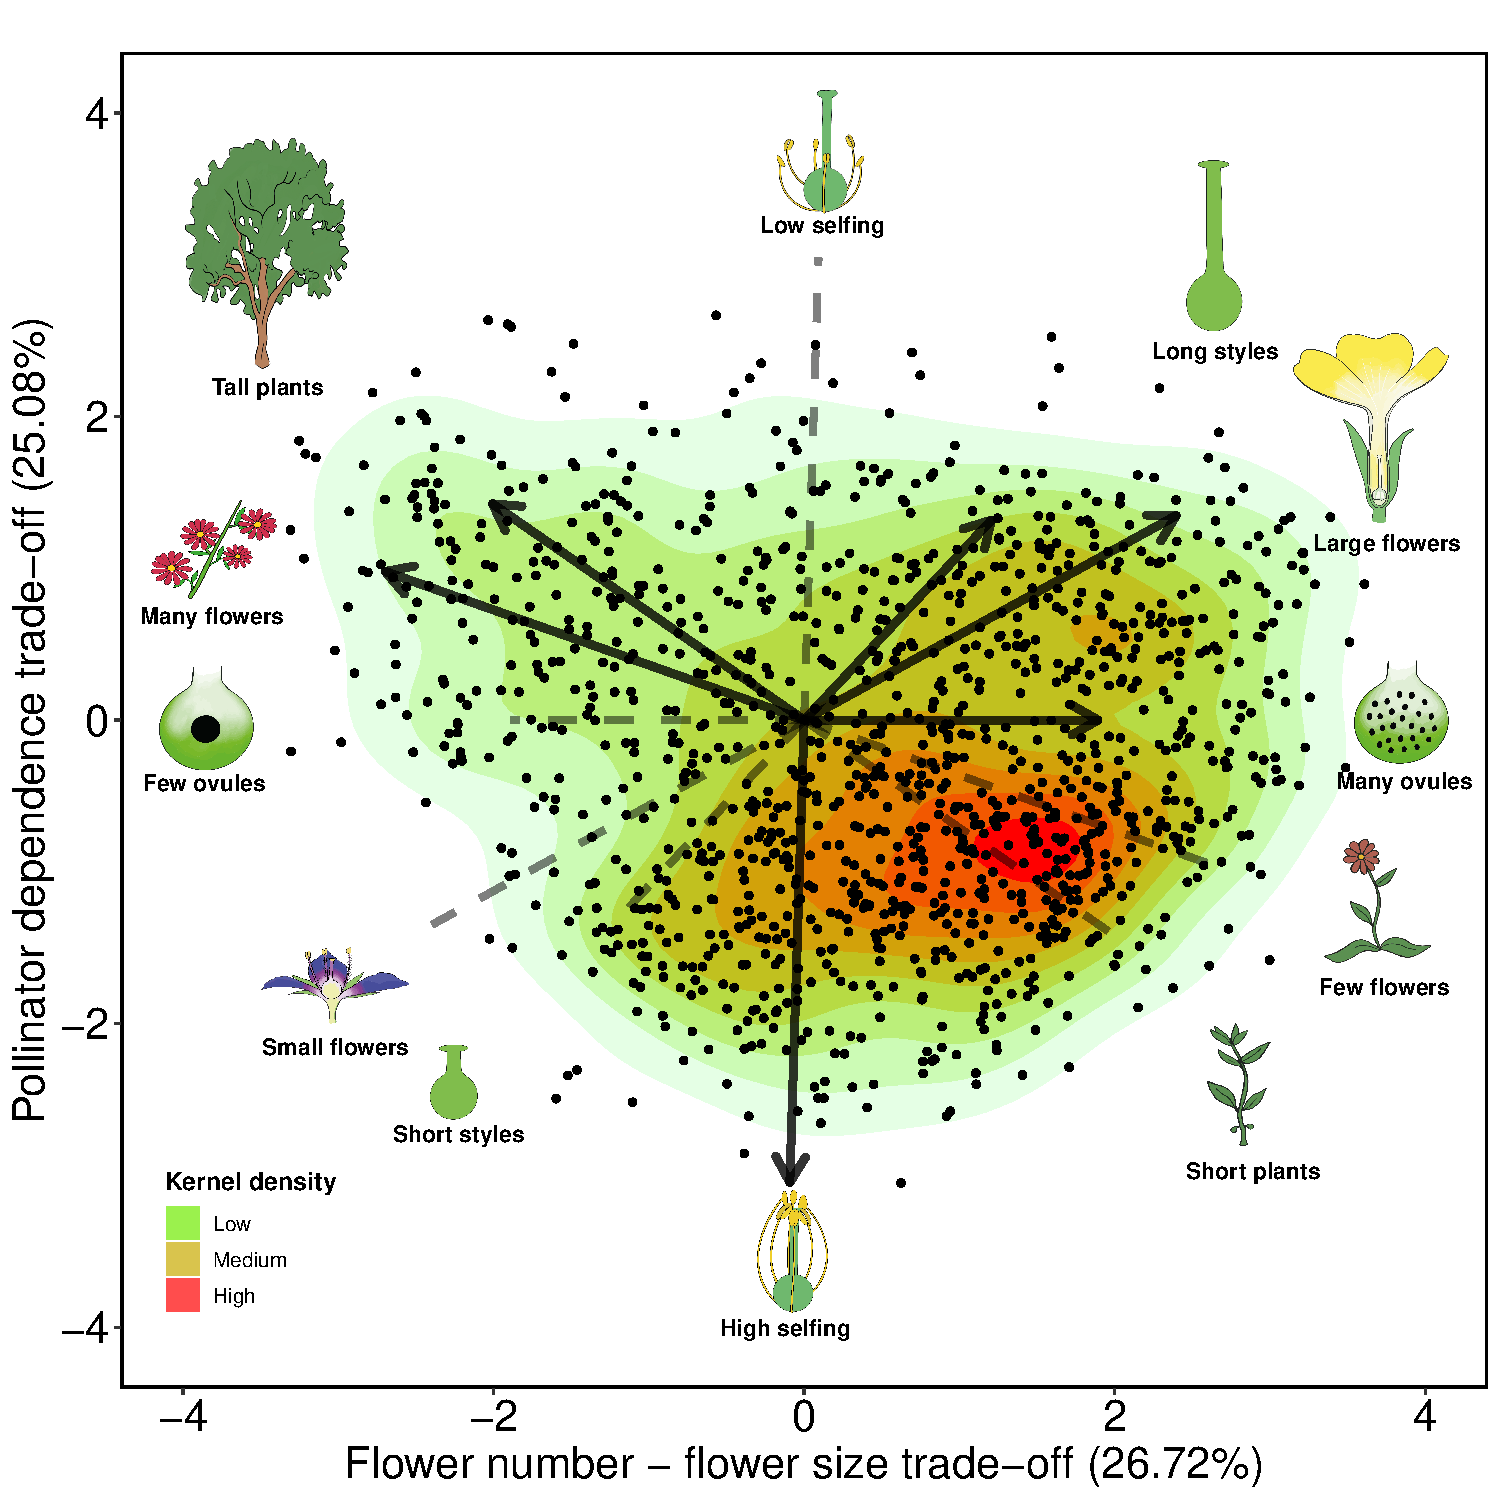
\includegraphics[width=0.85\linewidth]{output/figures/unnamed-chunk-2-1} 

}

\caption{\textbf{Figure 1.} Phylogenetically informed principal component analysis (pPCA) of 1,236 plant species from 28 plant-pollinator network studies. The solid arrows indicate the direction of the different quantitative traits (flower number, plant height, style length, flower size, ovule number and level of autonomous selfing) across the two main axes of trait variation. The length of the arrows indicate the weight of the variables on each principal component and the dashed lines show the opposed direction of trait variation. The icons at both ends of arrows and dashed lines illustrate the extreme form of the trait continuum.}\label{fig:unnamed-chunk-2}
\end{figure}

We found that most categorical traits were statistically associated with the first two axes of trait variation (figure 2 and table S2). Flower symmetry, which was only associated with PC2 (Sum of squares = 8.51, F-value = 14.72, \emph{P} \textless{} 0.01 ), and nectar provision, which was independent of PC1 and PC2 (PC1: Sum of squares = 0.37, F-value = 0.29 , \emph{P} = 0.59; PC2: Sum of squares = 0.83, F-value = 1.43, \emph{P} = 0.23) showed a lack of statistical association. In addition, we found statistical differences between the different categorical trait levels within the trait space (figure S7). Regarding self-compatibility, we found larger differences on PC2. For instance, species with unisexual flowers that were self-incompatible, were statistically differentiated from species with partial or full self-compatibility on this axis (figure S7a and figure S7b; Tukey test \emph{P} \textless{} 0.05). Life forms differed statistically across both axes of trait variation and followed a gradient of larger life forms (trees and shrubs) with lower autonomous selfing to smaller ones (herbs) with higher autonomous selfing (figure S7c and figure S7d; Tukey test \emph{P} \textless{} 0.05). Consequently, lifespan also followed this gradient but perennial and short lived species only differed statistically on PC2 (figure S7e and figure S7f; Tukey test \emph{P} \textless{} 0.05). Species with unisexual flowers (monoecious and dioecious) were clustered on both extremes of the first two principal components and had both the lowest autonomous selfing levels and the highest number of flowers (figure S7g and figure S7h; Tukey test \emph{P} \textless{} 0.05). Moreover, we found that campanulate and capitulum flower shapes were differentiated from tube, papilionaceous, open and brush shapes in the trait space; the former had larger flowers and low autonomous selfing levels, while the latter had more flowers and high autonomous selfing (figure S7i and figure S7j; Tukey test \emph{P} \textless{} 0.05). Finally, in terms of flower symmetry, zygomorphic flowers were associated with high levels of autonomous selfing, whereas actinomorphic flowers were more dependent on pollinators (figure S7k and figure S7l; Tukey test \emph{P} \textless{} 0.05).

\blandscape

\begin{figure}[H]

{\centering 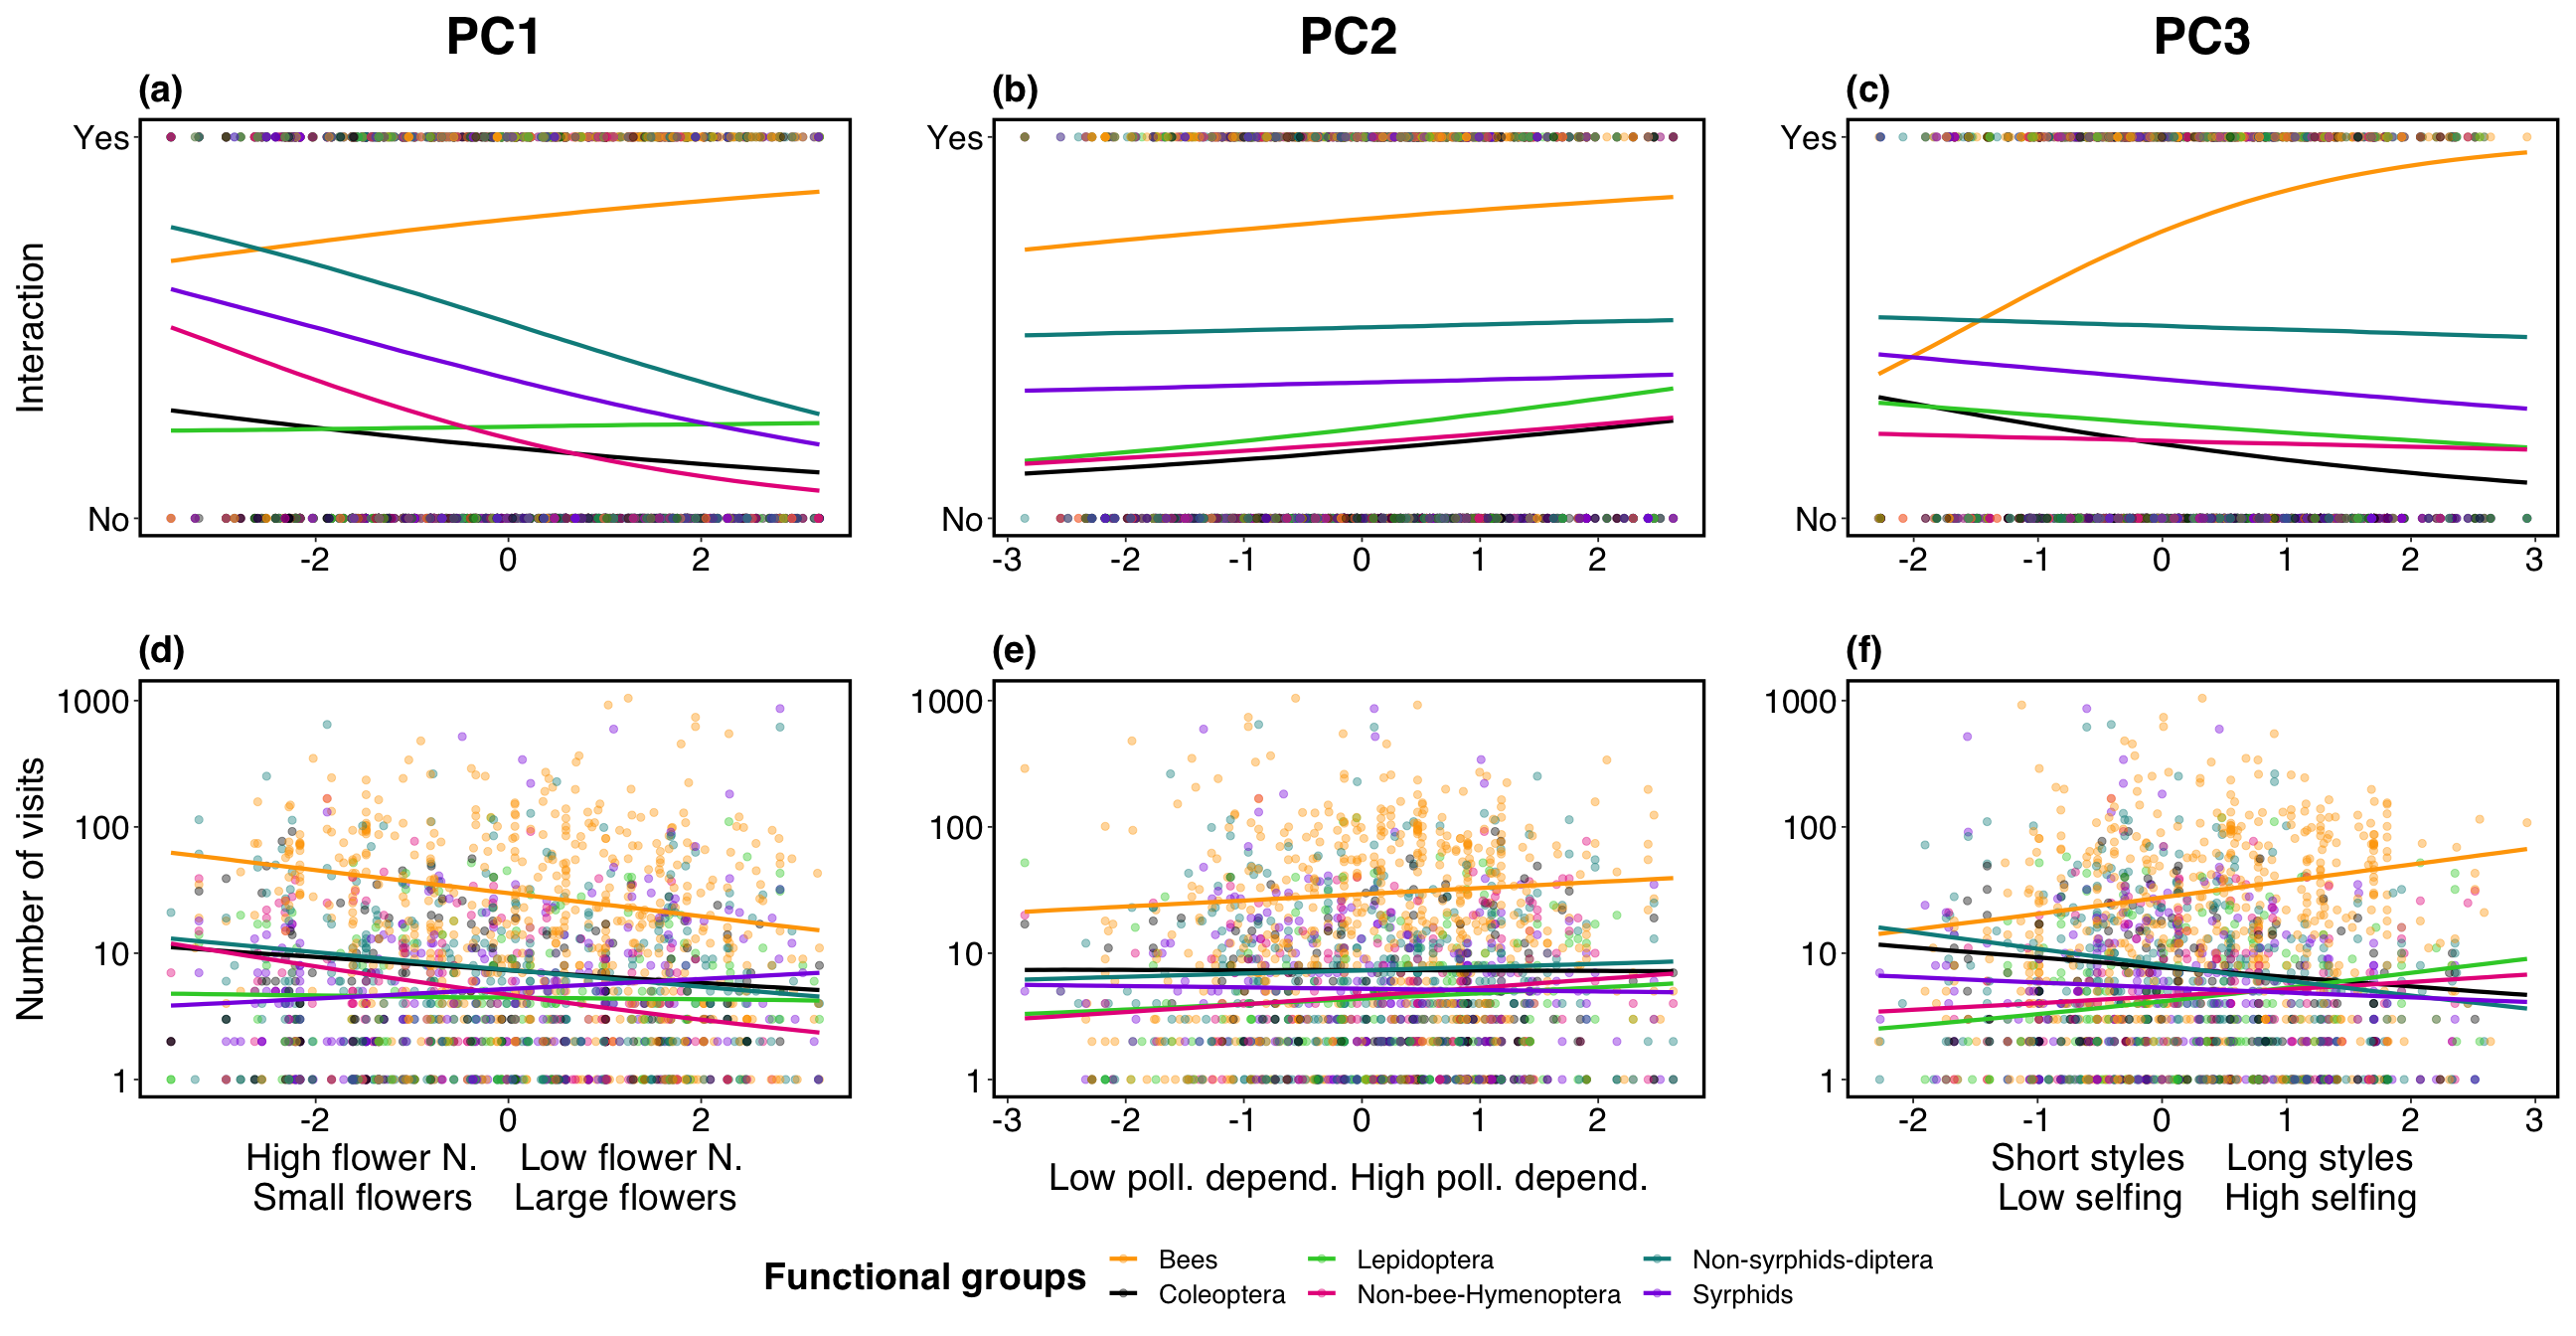
\includegraphics[width=0.8\linewidth]{output/figures/unnamed-chunk-3-1} 

}

\caption{\textbf{Figure 2.} Location of the different qualitative traits in the trait space. The figure panel is composed of the traits that showed statistical association with the first two axes of trait variation: compatibility system (a), life form (b), lifespan (c), breeding system (d), flower shape (e) and flower symmetry (f). The solid arrows indicate the direction of variation of the different quantitative traits shown in figure 1: flower number (FN), plant height (PH), style length (SL), flower size (FS), ovule number (ON) and the level of autonomous selfing (S).}\label{fig:unnamed-chunk-3}
\end{figure}

\elandscape

\hypertarget{b-phylogenetic-signal}{%
\subsection{(b) Phylogenetic signal}\label{b-phylogenetic-signal}}

We found a strong phylogenetic signal (\emph{P} \textless{} 0.01) for most quantitative traits (table S5). The traits that showed the highest phylogenetic signal were ovule number (\(\lambda\) = 1), pollen grains per flower (\(\lambda\) = 1) and plant height (\(\lambda\) = 0.96), followed by flower length (\(\lambda\) = 0.75), flower width (\(\lambda\) = 0.73), number of flowers per plant (\(\lambda\) = 0.69) and nectar concentration (\(\lambda\) = 0.65). The traits that had a moderate phylogenetic signal included inflorescence width (\(\lambda\) = 0.57), style length (\(\lambda\) = 0.49) and autonomous selfing (\(\lambda\) = 0.34). Finally, microliters of nectar per flower showed the lowest phylogenetic signal of all the traits we measured (\(\lambda\) = 0.14).

\hypertarget{c-visitation-patterns}{%
\subsection{(c) Visitation patterns}\label{c-visitation-patterns}}

The main axes of trait variation (PC1, PC2 and PC3) partly explained the presence-absence of interaction partners (conditional \(R^{2}\) = 0.26; marginal \(R^{2}\) = 0.20) but little of the total number of visits (conditional \(R^{2}\) = 0.31; marginal \(R^{2}\) = 0.06). However, we found relevant differences across the different pollinator guilds for both the presence-absence of interactions and number of visits (figure 3). On the flower number - flower size axis, we found that plants with many small flowers tended to have interaction partners that were Coleoptera, non-bee-Hymenoptera and Diptera (figure 3a), whereas plants with few large flowers mostly had interaction partners that were bees and Lepidoptera. We found similar trends for visitation rates on the flower number - flower size axis, but bees and syrphids visited plant species with many small flowers more frequently (figure 3d). On the autonomous selfing - floral display axis, we found that all plant species with lower autonomous selfing had many interaction partners and recieved many visits from all pollinator guilds (figure 3b and figure 3e). Finally, on the style length - autonomous selfing axis, plant species with short styles and low autonomous selfing had more interaction partners for all guilds, except bees which interacted more frequently with plant species with long styles and high autonomous selfing (figure 3c). Plants with long styles and high autonomous selfing interacted more frequently with Lepidoptera and non-bee-Hymenoptera (figure 3f).

The additional models for the most represented bee families, for both presence-absence of interactions (marginal \(R^{2}\) = 0.29; conditional \(R^{2}\) = 0.19) and the number of visits (marginal \(R^{2}\) = 0.30; conditional \(R^{2}\) = 0.03), showed that the Apidae family was the main driver of the observed patterns. The contrast between interaction presence/absence and number of visits for bees on PC1 (figure 3a and figure 3d) was driven by the Andrenidae family, which had more interaction partners but made fewer visits to plant species with few large flowers (figure S8).

\vspace{5mm}
\blandscape

\begin{figure}
\centering
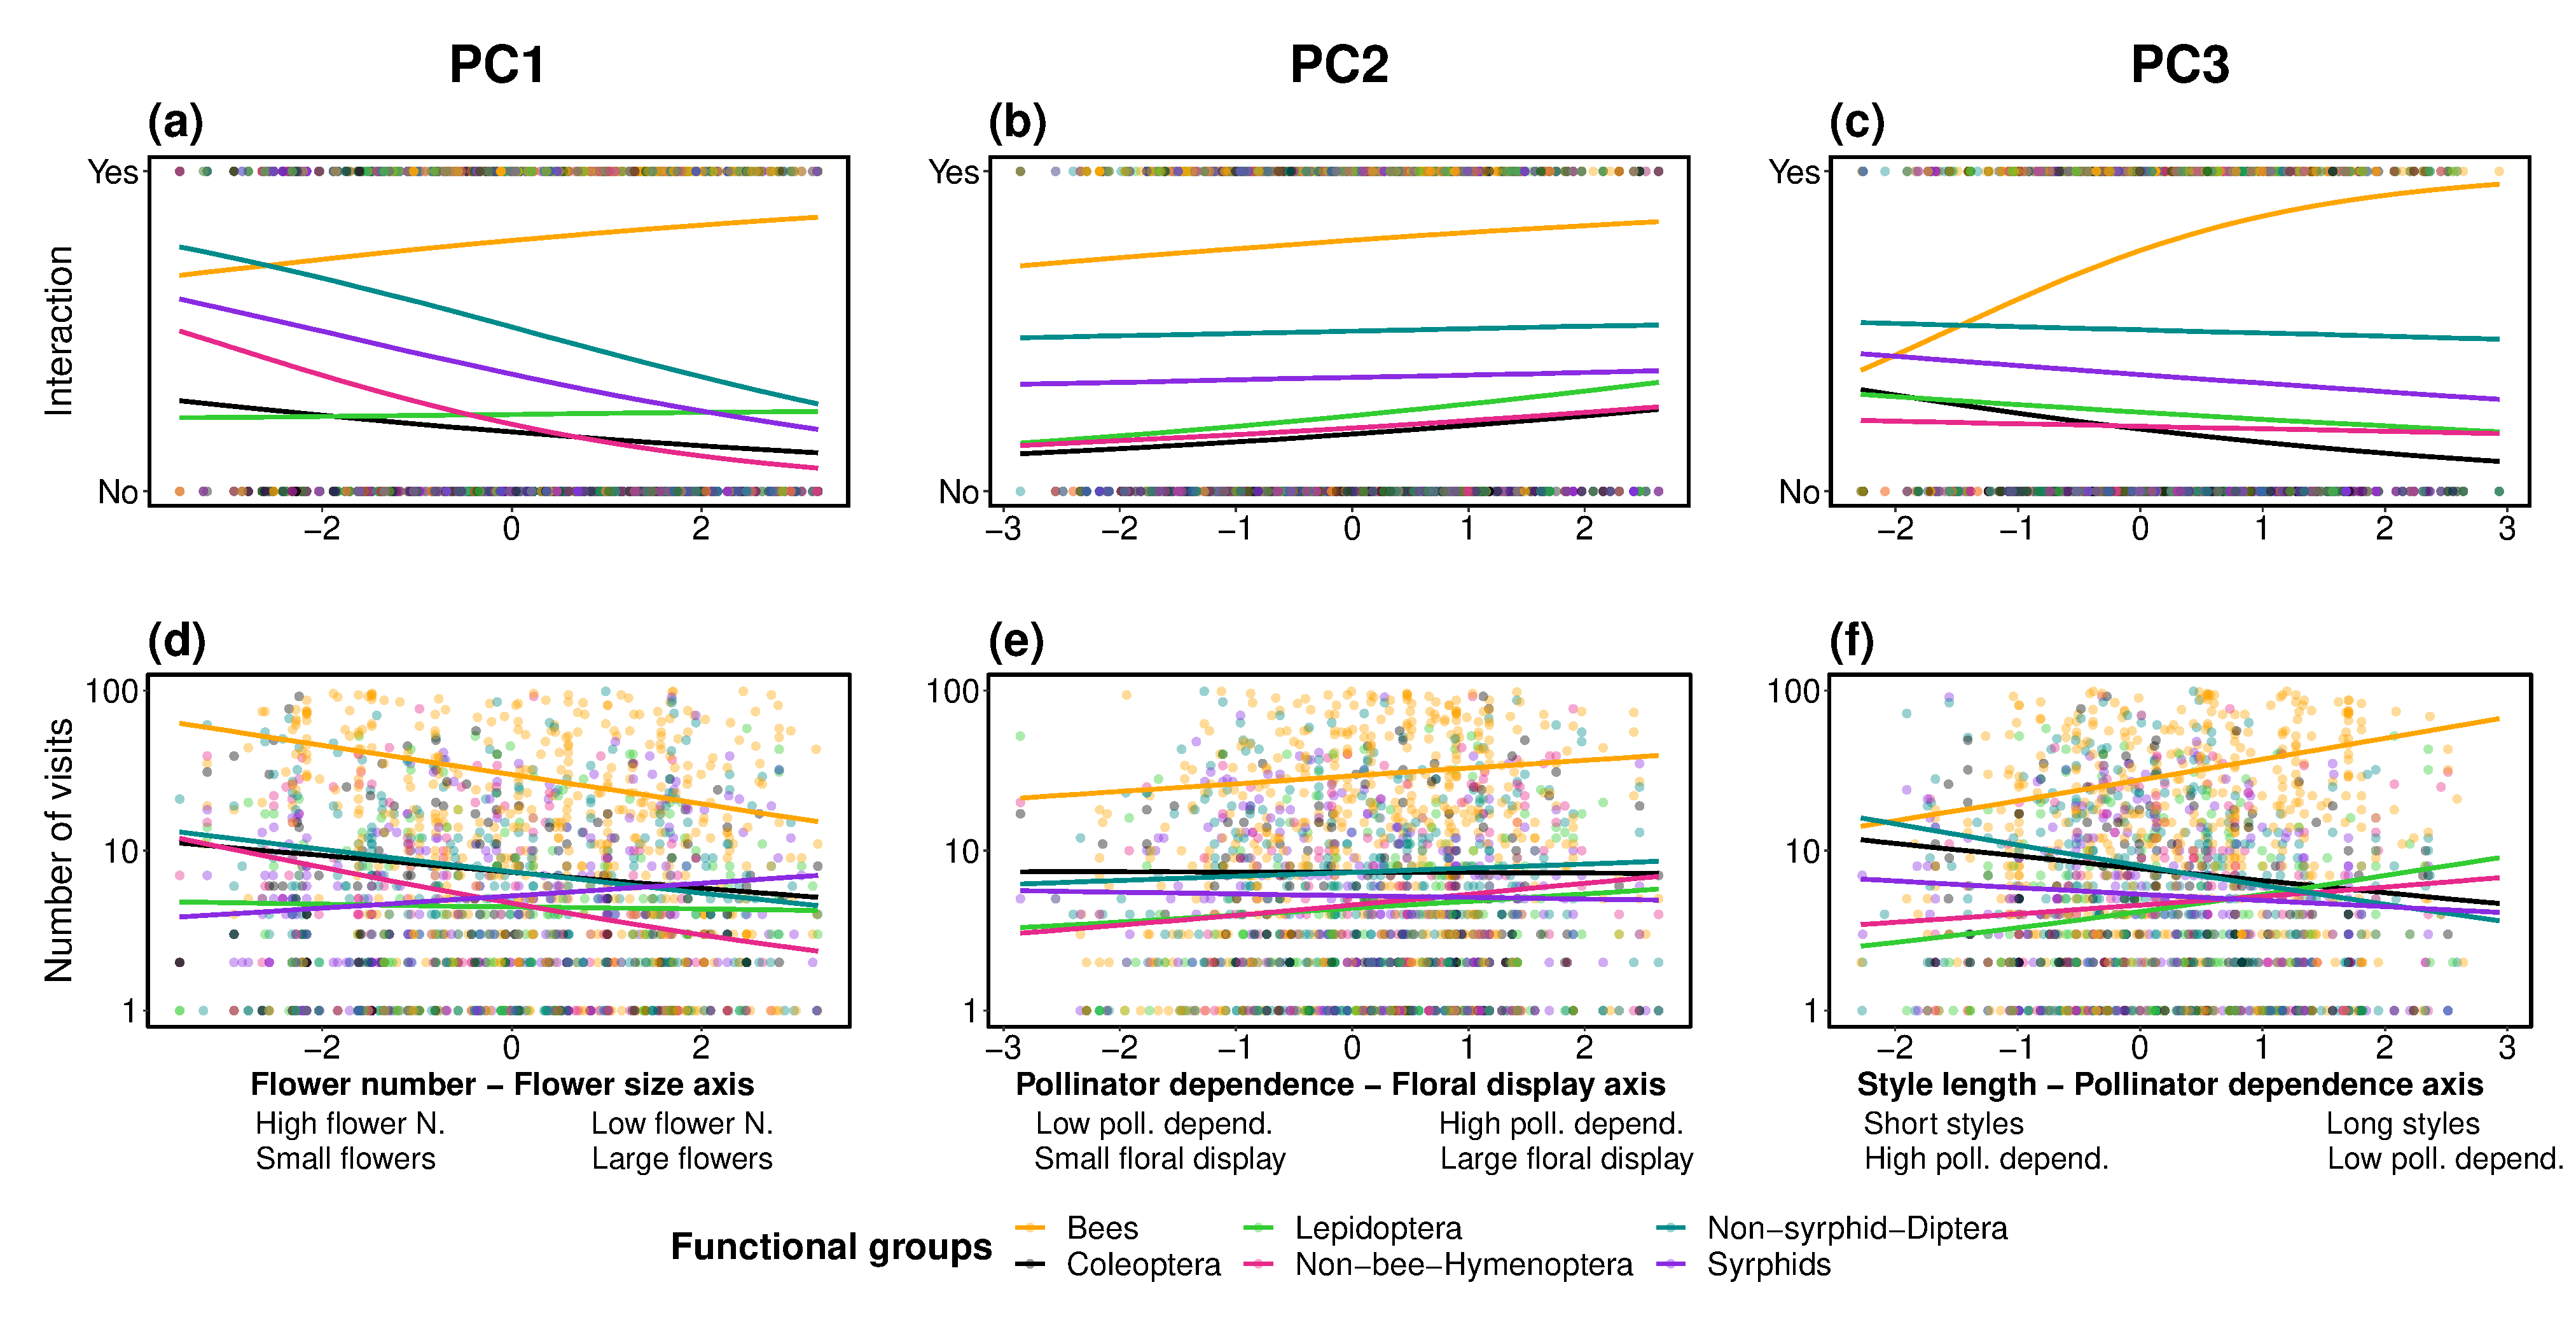
\includegraphics{output/figures/unnamed-chunk-4-1.pdf}
\caption{\label{fig:unnamed-chunk-4}\textbf{Figure 3.} Fitted posterior estimates of the presence-absence of interaction (a, b and c) and number of visits (d, e and f) of the different pollinator guilds in relation to the main axes of plant reproductive trait variation (PC1, PC2 and PC3). PC1 represents the flower number - flower size axis, PC2 represents the autonomous selfing - floral display axis and PC3 represents the style length - autonomous selfing axis. For visualization purposes due to large differences between number of visits from bees and the rest of the pollinator guilds, the number of visits was log-transformed (Y-axis of lower panel).}
\end{figure}

\elandscape

\hypertarget{d-plant-species-network-roles}{%
\subsection{(d) Plant species network roles}\label{d-plant-species-network-roles}}

Variance within plant species-level network metrics was poorly explained by the three main axes of trait variation (figure S9; number of visits \textasciitilde{} PCs, conditional \(R^{2}\) = 0.11, marginal \(R^{2}\) = 0.02; normalised degree \textasciitilde{} PCs, conditional \(R^{2}\) = 0.24, marginal \(R^{2}\) = 0.02; and, selectivity \textasciitilde{} PCs, conditional \(R^{2}\) = 0.37, marginal\(R^{2}\) = 0.03). Overall, the most notable trends were found on the flower number - flower size axis (PC1) and the style length - autonomous selfing axis (PC3) for number of visits and selectivity. On PC1, the number of visits per flower was higher for plant species with more flowers but was lower for plant species with larger flowers (figure S9a). However, selectivity (d') was higher for plant species with large flowers but lower for plant species with small flowers (figure S9g). On PC3, the number of visits was lower for plants with shorter styles and lower autonomous selfing but higher for plant species with longer styles and higher autonomous selfing (figure S9c). Again, selectivity showed the opposite trend to the number of visits (figure S9i).

\hypertarget{discussion}{%
\section{4. Discussion}\label{discussion}}

We found strong covariation among traits within the flowering plant reproductive spectrum, which shapes interactions with pollinators at a global scale. Despite the enormous variability in plant reproductive structures, the first two and three axes captured over 50\% and 70\% of trait variation, respectively, and these axes encapsulated correlations among flower number and flower size, autonomous selfing and floral display, and style length and autonomous selfing. Although explained trait variation on the first two axes was less than previous studies of morphological and physiological traits (\protect\hyperlink{ref-carmona2021}{Carmona et al., 2021}; \protect\hyperlink{ref-diaz2016}{Díaz et al., 2016}), our results align with the two largest and most recent studies of plant life strategies that included reproductive, form and size related traits (\protect\hyperlink{ref-vojtko2022}{E-Vojtkó et al., 2022}; \protect\hyperlink{ref-salguero2016}{Salguero-Gómez et al., 2016}). The different plant reproductive axes that we identified were associated with different numbers of interacting partners and visitation rates of the distinct pollinator guilds. However, the unexplained variability found highlights the need to account for other local factors, such as species relative abundances (\protect\hyperlink{ref-bartomeus2016}{Bartomeus et al., 2016}), along with reproductive traits, to better explain plant-pollinator associations.

Our study provides strong evidence for several widely discussed trait associations with the help of a great diversity of phylogenetic lineages (170 families and over 1,200 species). Specifically, by using a multitrait approach, we are able to link the reproductive spectrum of plant trait variation with the previously described ``fast-slow continuum'' in plant (\protect\hyperlink{ref-salguero2016}{Salguero-Gómez et al., 2016}) and animal (\protect\hyperlink{ref-healy2019}{Healy et al., 2019}) life-history strategies. This fast-slow continuum was illustrated by the associations between reproductive traits and plant height, life form and lifespan traits. For instance, although the negative correlation between flower number and flower size has received substantial attention (\protect\hyperlink{ref-kettle2011}{Kettle et al., 2011}; \protect\hyperlink{ref-sargent2007}{Sargent et al., 2007}; \protect\hyperlink{ref-worley2000}{Worley et al., 2000}), it has only been investigated across a few hundred Angiosperm species and generally lacking a multitrait perspective. We found support for this trait association and show that other reproductive traits (e.g., style length or ovule number) covary along this flower number - flower size axis. Our study also complements previous work linking plant breeding systems and life forms (\protect\hyperlink{ref-friedman2020}{Friedman, 2020}; \protect\hyperlink{ref-petit2006}{Petit \& Hampe, 2006}) by showing that most species with unisexual flowers also have woody life forms and many flowers. Moreover, we identify the previously documented positive association between outcrossing rate and floral display size (\protect\hyperlink{ref-goodwillie2010}{Goodwillie et al., 2010}), where species with low autonomous selfing levels also allocate large resource quantities to attract pollinators.

Although we did not include floral rewards in our main analysis due to insufficient data, we did find that plant species with large floral displays and, in particular, large flowers, tended to have higher pollen and nectar quantity. Thus, we demonstrate that globally, reproductive trait covariation in flowering plants likely imposes constraints on the broader spectrum of plant trait variation.

Overall, plant reproductive traits explained interaction patterns among and within pollinator guilds suggesting that plant reproductive strategies partly mediate these associations across spatial large scales. For example, we found that all pollinator guilds interacted more frequently with species with large floral displays and low ability to self pollinate, which aligns with previous findings (\protect\hyperlink{ref-hegland2005}{Hegland \& Totland, 2005}; \protect\hyperlink{ref-kaiser2014}{Kaiser-Bunbury et al., 2014}; \protect\hyperlink{ref-lazaro2013}{Lázaro et al., 2013}). As predicted by evolutionary life-history theory (\protect\hyperlink{ref-stebbins1970}{Stebbins, 1970}), larger investment in floral display and rewards to attract pollinators occurs when pollinator dependence is high. Indeed, the possible range of reproductive strategies in flowering plants is constrained by the cost of reproductive organs, trait associations and selective pressures exerted by different pollinator guilds (\protect\hyperlink{ref-galen1999}{Galen, 1999}). For instance, smaller flowers are visited less overall, but they are inexpensive to produce (e.g., have a low ovule number) and low visitation rate at the individual flower level can be compensated by overall visitation at the plant level by producing many flowers resulting in a larger quantity of small fruits (\protect\hyperlink{ref-kettle2011}{Kettle et al., 2011}). In addition, we found that a substantial number of species with high autonomous selfing had large styles and were associated with a high number of interactions with bees. These species seem to rely on animal pollinators as indicated by their high investment in sizable styles that can help prevent pollen competition (\protect\hyperlink{ref-ashman2013}{Ashman \& Arceo-Gómez, 2013}; \protect\hyperlink{ref-lanuza2021}{Lanuza et al., 2021}; \protect\hyperlink{ref-ramesha2011}{Ramesha et al., 2011}) while having reproductive assurance in their absence. For instance, the annual herb \emph{Scabiosa atropurpurea} has flowers grouped in clusters with relatively long styles and a single ovule per flower that is likely to be fertilised with a single legitimate floral visit but avoids reproductive failure with autonomous self pollination. Similarly, zygomorphic flowers are specialised floral structures that promote precise pollen transfer (\protect\hyperlink{ref-gong2009}{Gong \& Huang, 2009}; \protect\hyperlink{ref-sargent2004}{Sargent, 2004}) but they were associated with high levels of autogamy. Our findings are consistent with the idea that reproductive assurance is not rare within specialised pollination systems (\protect\hyperlink{ref-fenster2007}{Fenster \& Marten-Rodriguez, 2007}) and highlight the need to explore the timing (e.g., early versus delayed) and selfing mechanisms (see \protect\hyperlink{ref-goodwillie2018}{Goodwillie \& Weber, 2018}) in relation to other reproductive traits to better understand reproductive trait correlations and plant-pollinator interactions.

Because floral traits can be associated with their animal pollinators to optimise pollen transfer, the correlation between distinct suites of reproductive traits and pollinator guilds could indicate the existence of pollination syndromes (\protect\hyperlink{ref-dellinger2020}{Dellinger, 2020}; \protect\hyperlink{ref-faegri2013}{Faegri \& Van Der Pijl, 2013}; \protect\hyperlink{ref-fenster2004}{Fenster et al., 2004}; \protect\hyperlink{ref-rosas2014}{Rosas-Guerrero et al., 2014}). For instance, bees had a higher number of interacting partners on plant species with large flowers but interacted more frequently with species with small flowers while syrphid flies showed the opposite trend. This could be reflective of differences in the ecology and behaviour between these pollinator guilds (\protect\hyperlink{ref-foldesi2021}{Földesi et al., 2021}; \protect\hyperlink{ref-rader2020}{Rader et al., 2020}) that ultimately exert different selective pressures, leading divergent plant reproductive strategies. In any case, it is worth noting that local factors (e.g., species relative abundances or phenologies) likely contribute to the variability in the association between the plant reproductive spectrum and pollinators (\protect\hyperlink{ref-bartomeus2016}{Bartomeus et al., 2016}; \protect\hyperlink{ref-encinas2012}{Encinas-Viso et al., 2012}; \protect\hyperlink{ref-vazquez2007}{Vázquez et al., 2007}). Taking both aspects together, we suggest that while plant reproductive traits do shape their interactions with pollinators, pollinator syndromes at a macroecological scale are not distinct compartmentalised items, but form part of a multifaceted context dependent continuum.

Our study provides a comprehensive assessment of reproductive trait covariation patterns in flowering plants, using a global dataset of traits for plant species within plant-pollinator networks. We show the importance of pollinators in mediating reproductive trait correlations and identify the need to consider broader plant reproductive strategies, rather than just flower morphology, to understand patterns of plant-pollinator interactions. Further, we provide empirical evidence of reproductive trait associations that complement trait covariation studies for other plant organs, highlighting the need to include reproductive traits in the global spectrum of plant form and function. Future work incorporating underrepresented areas of the world and additional relevant reproductive traits (e.g., flower life span and colour) from a broader range of life forms will be valuable for enhancing our understanding of the plant reproductive spectrum and associated plant-pollinator interactions.

\newpage

\hypertarget{references}{%
\section{References}\label{references}}

\hypertarget{refs}{}
\begin{CSLReferences}{1}{0}
\leavevmode\vadjust pre{\hypertarget{ref-abdi2010}{}}%
Abdi, H., \& Williams, L. J. (2010). Principal component analysis. \emph{WIREs Comp. Stats.}, \emph{2}(4), 433--459. \url{https://doi.org/10.1002/wics.101}

\leavevmode\vadjust pre{\hypertarget{ref-agrawal2020}{}}%
Agrawal, A. A. (2020). A scale-dependent framework for trade-offs, syndromes, and specialization in organismal biology. \emph{Ecology}, \emph{101}(2), e02924. \url{https://doi.org/10.1002/ecy.2924}

\leavevmode\vadjust pre{\hypertarget{ref-ashman2013}{}}%
Ashman, T.-L., \& Arceo-Gómez, G. (2013). Toward a predictive understanding of the fitness costs of heterospecific pollen receipt and its importance in co-flowering communities. \emph{American Journal of Botany}, \emph{100}(6), 1061--1070. \url{https://doi.org/10.3732/ajb.1200496}

\leavevmode\vadjust pre{\hypertarget{ref-ballantyne2015}{}}%
Ballantyne, G., Baldock, K. C. R., \& Willmer, P. G. (2015). Constructing more informative plant\textendash pollinator networks: Visitation and pollen deposition networks in a heathland plant community. \emph{Proc. Royal Soc. B}, \emph{282}(1814), 20151130. \url{https://doi.org/10.1098/rspb.2015.1130}

\leavevmode\vadjust pre{\hypertarget{ref-barrett2002}{}}%
Barrett, S. C. H. (2002). The evolution of plant sexual diversity. \emph{Nat. Rev. Genet.}, \emph{3}(4), 274--284. \url{https://doi.org/10.1038/nrg776}

\leavevmode\vadjust pre{\hypertarget{ref-barrett2003}{}}%
Barrett, S. C. H. (2003). Mating strategies in flowering plants: The outcrossing-selfing paradigm and beyond. \emph{Philos. Trans. R. Soc. Lond. B Biol. Sci.}, \emph{358}(1434), 991--1004. \url{https://doi.org/10.1098/rstb.2003.1301}

\leavevmode\vadjust pre{\hypertarget{ref-bartomeus2016}{}}%
Bartomeus, I., Gravel, D., Tylianakis, J. M., Aizen, M. A., Dickie, I. A., \& Bernard-Verdier, M. (2016). A common framework for identifying linkage rules across different types of interactions. \emph{Funct. Ecol.}, \emph{30}(12), 1894--1903. \url{https://doi.org/10.1111/1365-2435.12666}

\leavevmode\vadjust pre{\hypertarget{ref-bluthgen2006}{}}%
Blüthgen, N., Menzel, F., \& Blüthgen, N. (2006). Measuring specialization in species interaction networks. \emph{BMC Ecol.}, \emph{6}(1), 9. \url{https://doi.org/10.1186/1472-6785-6-9}

\leavevmode\vadjust pre{\hypertarget{ref-bruelheide2018}{}}%
Bruelheide, H., Dengler, J., Purschke, O., Lenoir, J., Jiménez-Alfaro, B., Hennekens, S. M., Botta-Dukát, Z., Chytry, M., Field, R., Jansen, F., et al. (2018). Global trait--environment relationships of plant communities. \emph{Nat. Ecol. Evol.}, \emph{2}(12), 1906--1917. \url{https://doi.org/10.1038/s41559-018-0699-8}

\leavevmode\vadjust pre{\hypertarget{ref-burkner2017}{}}%
Bürkner, P.-C. (2017). Brms: {An R} package for {Bayesian} multilevel models using {Stan}. \emph{J. Stat. Softw.}, \emph{80}(1), 1--28. \url{https://doi.org/10.18637/jss.v080.i01}

\leavevmode\vadjust pre{\hypertarget{ref-carmona2021}{}}%
Carmona, C. P., Tamme, R., Pärtel, M., Bello, F. de, Brosse, S., Capdevila, P., González-M, R., González-Suárez, M., Salguero-Gómez, R., Vásquez-Valderrama, M., \& Toussaint, A. (2021). Erosion of global functional diversity across the tree of life. \emph{Sci. Adv.}, \emph{7}(13), eabf2675. \url{https://doi.org/10.1126/sciadv.abf2675}

\leavevmode\vadjust pre{\hypertarget{ref-carvalheiro2014}{}}%
Carvalheiro, L. G., Biesmeijer, J. C., Benadi, G., Fründ, J., Stang, M., Bartomeus, I., Kaiser-Bunbury, C. N., Baude, M., Gomes, S. I. F., Merckx, V., Baldock, K. C. R., Bennett, A. T. D., Boada, R., Bommarco, R., Cartar, R., Chacoff, N., Dänhardt, J., Dicks, L. V., Dormann, C. F., \ldots{} Kunin, W. E. (2014). The potential for indirect effects between co-flowering plants via shared pollinators depends on resource abundance, accessibility and relatedness. \emph{Ecol. Lett.}, \emph{17}(11), 1389--1399. \url{https://doi.org/10.1111/ele.12342}

\leavevmode\vadjust pre{\hypertarget{ref-santos2018}{}}%
Chamberlain, S., Szoecs, E., Foster, Z., Arendsee, Z., Boettiger, C., Ram, K., Bartomeus, I., Baumgartner, J., O'Donnell, J., Oksanen, J., Tzovaras, B. G., Marchand, P., Tran, V., Salmon, M., Li, G., \& Grenié, M. (2018). \emph{Package {``{PVR}.''} R package version 0.3.~At \href{https://CRAN.R-project.org/package=PVR}{https://CRAN.r-project.org/package=PVR}}.

\leavevmode\vadjust pre{\hypertarget{ref-chamberlain2020}{}}%
Chamberlain, S., Szoecs, E., Foster, Z., Arendsee, Z., Boettiger, C., Ram, K., Bartomeus, I., Baumgartner, J., O'Donnell, J., Oksanen, J., Tzovaras, B. G., Marchand, P., Tran, V., Salmon, M., Li, G., \& Grenié, M. (2020). \emph{Taxize: {Taxonomic} information from around the web. R package version 0.9.99.~At \href{https://CRAN.R-project.org/package=taxize}{https://CRAN.r-project.org/package=taxize}}.

\leavevmode\vadjust pre{\hypertarget{ref-chave2009}{}}%
Chave, J., Coomes, D., Jansen, S., Lewis, S. L., Swenson, N. G., \& Zanne, A. E. (2009). Towards a worldwide wood economics spectrum. \emph{Ecol. Lett.}, \emph{12}(4), 351--366. \url{https://doi.org/10.1111/j.1461-0248.2009.01285.x}

\leavevmode\vadjust pre{\hypertarget{ref-coux2016}{}}%
Coux, C., Rader, R., Bartomeus, I., \& Tylianakis, J. M. (2016). Linking species functional roles to their network roles. \emph{Ecol. Lett.}, \emph{19}(7), 762--770. \url{https://doi.org/10.1111/ele.12612}

\leavevmode\vadjust pre{\hypertarget{ref-dehling2016}{}}%
Dehling, D. M., Jordano, P., Schaefer, H. M., Böhning-Gaese, K., \& Schleuning, M. (2016). Morphology predicts species' functional roles and their degree of specialization in plant--frugivore interactions. \emph{Proc. Royal Soc. B}, \emph{283}(1823), 20152444. \url{https://doi.org/10.1098/rspb.2015.2444}

\leavevmode\vadjust pre{\hypertarget{ref-dellinger2020}{}}%
Dellinger, A. S. (2020). Pollination syndromes in the 21st century: Where do we stand and where may we go? \emph{New Phytol.}, \emph{228}(4), 1193--1213. \url{https://doi.org/10.1111/nph.16793}

\leavevmode\vadjust pre{\hypertarget{ref-devaux2014}{}}%
Devaux, C., Lepers, C., \& Porcher, E. (2014). Constraints imposed by pollinator behaviour on the ecology and evolution of plant mating systems. \emph{J. Evol. Biol.}, \emph{27}(7), 1413--1430. \url{https://doi.org/10.1111/jeb.12380}

\leavevmode\vadjust pre{\hypertarget{ref-diaz2016}{}}%
Díaz, S., Kattge, J., Cornelissen, J. H. C., Wright, I. J., Lavorel, S., Dray, S., Reu, B., Kleyer, M., Wirth, C., Colin Prentice, I., Garnier, E., Bönisch, G., Westoby, M., Poorter, H., Reich, P. B., Moles, A. T., Dickie, J., Gillison, A. N., Zanne, A. E., \ldots{} Gorné, L. D. (2016). The global spectrum of plant form and function. \emph{Nature}, \emph{529}(7585), 167--171. \url{https://doi.org/10.1038/nature16489}

\leavevmode\vadjust pre{\hypertarget{ref-diniz-filho2012}{}}%
Diniz-Filho, J. A. F., Bini, L. M., Rangel, T. F., Morales-Castilla, I., Olalla-Tárraga, M. Á., Rodríguez, M. Á., \& Hawkins, B. A. (2012). On the selection of phylogenetic eigenvectors for ecological analyses. \emph{Ecography}, \emph{35}(3), 239--249. \url{https://doi.org/10.1111/j.1600-0587.2011.06949.x}

\leavevmode\vadjust pre{\hypertarget{ref-donovan2011}{}}%
Donovan, L. A., Maherali, H., Caruso, C. M., Huber, H., \& Kroon, H. de. (2011). The evolution of the worldwide leaf economics spectrum. \emph{Trends in Ecology \& Evolution}, \emph{26}(2), 88--95. \url{https://doi.org/10.1016/j.tree.2010.11.011}

\leavevmode\vadjust pre{\hypertarget{ref-dormann2008}{}}%
Dormann, C. F., Gruber, B., \& Fründ, J. (2008). Introducing the bipartite package: Analysing ecological networks. \emph{R News}, \emph{8/2}.

\leavevmode\vadjust pre{\hypertarget{ref-eklof2013}{}}%
Eklöf, A., Jacob, U., Kopp, J., Bosch, J., Castro-Urgal, R., Chacoff, N. P., Dalsgaard, B., Sassi, C. de, Galetti, M., Guimaraes, P. R., et al. (2013). The dimensionality of ecological networks. \emph{Ecol. Lett.}, \emph{16}(5), 577--583. \url{https://doi.org/10.1111/ele.12081}

\leavevmode\vadjust pre{\hypertarget{ref-encinas2012}{}}%
Encinas-Viso, F., Revilla, T. A., \& Etienne, R. S. (2012). Phenology drives mutualistic network structure and diversity. \emph{Ecol. Lett.}, \emph{15}(3), 198--208. \url{https://doi.org/10.1111/j.1461-0248.2011.01726.x}

\leavevmode\vadjust pre{\hypertarget{ref-evojtko2020}{}}%
E-Vojtkó, A., Bello, F. de, Durka, W., Kühn, I., \& Götzenberger, L. (2020). The neglected importance of floral traits in trait-based plant community assembly. \emph{J. Veg. Sci.}, \emph{31}(4), 529--539. \url{https://doi.org/10.1111/jvs.12877}

\leavevmode\vadjust pre{\hypertarget{ref-vojtko2022}{}}%
E-Vojtkó, A., Junker, R. R., Bello, F. de, \& Götzenberger, L. (2022). Floral and reproductive traits are an independent dimension within the plant economic spectrum of temperate central europe. \emph{New Phytologist}. \url{https://doi.org/10.1111/nph.18386}

\leavevmode\vadjust pre{\hypertarget{ref-faegri2013}{}}%
Faegri, K., \& Van Der Pijl, L. (2013). \emph{Principles of pollination ecology} ({3rd edn}). {Elsevier}.

\leavevmode\vadjust pre{\hypertarget{ref-fenster2004}{}}%
Fenster, C. B., Armbruster, W. S., Wilson, P., Dudash, M. R., \& Thomson, J. D. (2004). Pollination {Syndromes} and {Floral Specialization}. \emph{Annu. Rev. Ecol. Evol. Syst.}, \emph{35}(1), 375--403. \url{https://doi.org/10.1146/annurev.ecolsys.34.011802.132347}

\leavevmode\vadjust pre{\hypertarget{ref-fenster2007}{}}%
Fenster, C. B., \& Marten-Rodriguez, S. (2007). Reproductive assurance and the evolution of pollination specialization. \emph{International Journal of Plant Sciences}, \emph{168}(2), 215--228. \url{https://doi.org/10.1086/509647}

\leavevmode\vadjust pre{\hypertarget{ref-foldesi2021}{}}%
Földesi, R., Howlett, B. G., Grass, I., \& Batáry, P. (2021). Larger pollinators deposit more pollen on stigmas across multiple plant species---a meta-analysis. \emph{J. Appl. Ecol.}, \emph{58}(4), 699--707. \url{https://doi.org/10.1111/1365-2664.13798}

\leavevmode\vadjust pre{\hypertarget{ref-fortuna2010}{}}%
Fortuna, M. A., Stouffer, D. B., Olesen, J. M., Jordano, P., Mouillot, D., Krasnov, B. R., Poulin, R., \& Bascompte, J. (2010). Nestedness versus modularity in ecological networks: Two sides of the same coin? \emph{J. Anim. Ecol.}, \emph{79}(4), 811--817. \url{https://doi.org/10.1111/j.1365-2656.2010.01688.x}

\leavevmode\vadjust pre{\hypertarget{ref-friedman2020}{}}%
Friedman, J. (2020). The evolution of annual and perennial plant life histories: Ecological correlates and genetic mechanisms. \emph{Annu. Rev. Ecol. Evol. Syst.}, \emph{51}, 461--481. \url{https://doi.org/10.1146/annurev-ecolsys-110218-024638}

\leavevmode\vadjust pre{\hypertarget{ref-gabry2019}{}}%
Gabry, J., Simpson, D., Vehtari, A., Betancourt, M., \& Gelman, A. (2019). Visualization in {Bayesian} workflow. \emph{J. R. Stat. Soc. Ser. A Stat. Soc.}, \emph{182}(2), 389--402. \url{https://doi.org/10.1111/rssa.12378}

\leavevmode\vadjust pre{\hypertarget{ref-galen1999}{}}%
Galen, C. (1999). Why do flowers vary? The functional ecology of variation in flower size and form within natural plant populations. \emph{Bioscience}, \emph{49}(8), 631--640. \url{https://doi.org/10.2307/1313439}

\leavevmode\vadjust pre{\hypertarget{ref-gong2009}{}}%
Gong, Y.-B., \& Huang, S.-Q. (2009). Floral symmetry: Pollinator-mediated stabilizing selection on flower size in bilateral species. \emph{Proceedings of the Royal Society B: Biological Sciences}, \emph{276}(1675), 4013--4020. \url{https://doi.org/10.1098/rspb.2009.1254}

\leavevmode\vadjust pre{\hypertarget{ref-goodwillie2010}{}}%
Goodwillie, C., Sargent, R. D., Eckert, C. G., Elle, E., Geber, M. A., Johnston, M. O., Kalisz, S., Moeller, D. A., Ree, R. H., Vallejo-Marin, M., \& Winn, A. A. (2010). Correlated evolution of mating system and floral display traits in flowering plants and its implications for the distribution of mating system variation. \emph{New Phytol.}, \emph{185}(1), 311--321. \url{https://doi.org/10.1111/j.1469-8137.2009.03043.x}

\leavevmode\vadjust pre{\hypertarget{ref-goodwillie2018}{}}%
Goodwillie, C., \& Weber, J. J. (2018). The best of both worlds? A review of delayed selfing in flowering plants. \emph{American Journal of Botany}, \emph{105}(4), 641--655. \url{https://doi.org/10.1002/ajb2.1045}

\leavevmode\vadjust pre{\hypertarget{ref-healy2019}{}}%
Healy, K., Ezard, T. H. G., Jones, O. R., Salguero-Gómez, R., \& Buckley, Y. M. (2019). Animal life history is shaped by the pace of life and the distribution of age-specific mortality and reproduction. \emph{Nat. Ecol. Evol.}, \emph{3}(8), 1217--1224. \url{https://doi.org/10.1038/s41559-019-0938-7}

\leavevmode\vadjust pre{\hypertarget{ref-hegland2005}{}}%
Hegland, S. J., \& Totland, Ø. (2005). Relationships between species' floral traits and pollinator visitation in a temperate grassland. \emph{Oecologia}, \emph{145}(4), 586--594. \url{https://doi.org/10.1007/s00442-005-0165-6}

\leavevmode\vadjust pre{\hypertarget{ref-hung2018}{}}%
Hung, K.-L. J., Kingston, J. M., Albrecht, M., Holway, D. A., \& Kohn, J. R. (2018). The worldwide importance of honey bees as pollinators in natural habitats. \emph{Proc. Royal Soc. B}, \emph{285}(1870), 20172140. \url{https://doi.org/10.1098/rspb.2017.2140}

\leavevmode\vadjust pre{\hypertarget{ref-ibanez2012}{}}%
Ibanez, S. (2012). Optimizing size thresholds in a plant-pollinator interaction web: Towards a mechanistic understanding of ecological networks. \emph{Oecologia}, \emph{170}(1), 233--242. \url{https://doi.org/10.1007/s00442-012-2290-3}

\leavevmode\vadjust pre{\hypertarget{ref-jin2019}{}}%
Jin, Y., \& Qian, H. (2019). V.{PhyloMaker}: An {R} package that can generate very large phylogenies for vascular plants. \emph{Ecography}, \emph{42}(8), 1353--1359. \url{https://doi.org/10.1111/ecog.04434}

\leavevmode\vadjust pre{\hypertarget{ref-junker2013}{}}%
Junker, R. R., Blüthgen, N., Brehm, T., Binkenstein, J., Paulus, J., Schaefer, H. M., \& Stang, M. (2013). Specialization on traits as basis for the niche-breadth of flower visitors and as structuring mechanism of ecological networks. \emph{Funct. Ecol.}, \emph{27}(2), 329--341. \url{https://doi.org/10.1111/1365-2435.12005}

\leavevmode\vadjust pre{\hypertarget{ref-kaiser2014}{}}%
Kaiser-Bunbury, C. N., Vázquez, D. P., Stang, M., \& Ghazoul, J. (2014). Determinants of the microstructure of plant\textendash pollinator networks. \emph{Ecology}, \emph{95}(12), 3314--3324. \url{https://doi.org/10.1890/14-0024.1}

\leavevmode\vadjust pre{\hypertarget{ref-kattge2011}{}}%
Kattge, J., Díaz, S., Lavorel, S., Prentice, I. C., Leadley, P., Bönisch, G., Garnier, E., Westoby, M., Reich, P. B., Wright, I. J., Cornelissen, J. H. C., Violle, C., Harrison, S. P., Bodegom, P. M. V., Reichstein, M., Enquist, B. J., Soudzilovskaia, N. A., Ackerly, D. D., Anand, M., \ldots{} Wirth, C. (2011). {TRY} \textendash{} a global database of plant traits. \emph{Glob. Chang. Biol.}, \emph{17}(9), 2905--2935. \url{https://doi.org/10.1111/j.1365-2486.2011.02451.x}

\leavevmode\vadjust pre{\hypertarget{ref-kettle2011}{}}%
Kettle, C. J., Maycock, C. R., Ghazoul, J., Hollingsworth, P. M., Khoo, E., Sukri, R. S. H., \& Burslem, D. F. R. P. (2011). Ecological {Implications} of a {Flower Size}/{Number Trade}-{Off} in {Tropical Forest Trees}. \emph{PLoS One}, \emph{6}(2), e16111. \url{https://doi.org/10.1371/journal.pone.0016111}

\leavevmode\vadjust pre{\hypertarget{ref-lanuza2021}{}}%
Lanuza, J. B., Bartomeus, I., Ashman, T.-L., Bible, G., \& Rader, R. (2021). Recipient and donor characteristics govern the hierarchical structure of heterospecific pollen competition networks. \emph{Journal of Ecology}, \emph{109}(6), 2329--2341. \url{https://doi.org/10.1111/1365-2745.13640}

\leavevmode\vadjust pre{\hypertarget{ref-laughlin2021}{}}%
Laughlin, D. C., Mommer, L., Sabatini, F. M., Bruelheide, H., Kuyper, T. W., McCormack, M. L., Bergmann, J., Freschet, G. T., Guerrero-Ramírez, N. R., Iversen, C. M., et al. (2021). Root traits explain plant species distributions along climatic gradients yet challenge the nature of ecological trade-offs. \emph{Nat. Ecol. Evol.}, 1--12. \url{https://doi.org/10.1038/s41559-021-01471-7}

\leavevmode\vadjust pre{\hypertarget{ref-lazaro2013}{}}%
Lázaro, A., Jakobsson, A., \& Totland, Ø. (2013). How do pollinator visitation rate and seed set relate to species' floral traits and community context? \emph{Oecologia}, \emph{173}(3), 881--893. \url{https://doi.org/10.1007/s00442-013-2652-5}

\leavevmode\vadjust pre{\hypertarget{ref-legendre2012}{}}%
Legendre, P., \& Legendre, L. (2012). \emph{Numerical ecology} ({2nd edn}). {Elsevier, Amsterdam}.

\leavevmode\vadjust pre{\hypertarget{ref-moeller2017}{}}%
Moeller, D. A., Runquist, R. D. B., Moe, A. M., Geber, M. A., Goodwillie, C., Cheptou, P.-O., Eckert, C. G., Elle, E., Johnston, M. O., Kalisz, S., Ree, R. H., Sargent, R. D., Vallejo-Marin, M., \& Winn, A. A. (2017). Global biogeography of mating system variation in seed plants. \emph{Ecol. Lett.}, \emph{20}(3), 375--384. \url{https://doi.org/10.1111/ele.12738}

\leavevmode\vadjust pre{\hypertarget{ref-munoz2016}{}}%
Munoz, F., Violle, C., \& Cheptou, P.-O. (2016). {CSR} ecological strategies and plant mating systems: Outcrossing increases with competitiveness but stress-tolerance is related to mixed mating. \emph{Oikos}, \emph{125}(9), 1296--1303. \url{https://doi.org/10.1111/oik.02328}

\leavevmode\vadjust pre{\hypertarget{ref-olesen2007}{}}%
Olesen, J. M., Bascompte, J., Dupont, Y. L., \& Jordano, P. (2007). The modularity of pollination networks. \emph{PNAS}, \emph{104}(50), 19891--19896. \url{https://doi.org/10.1073/pnas.0706375104}

\leavevmode\vadjust pre{\hypertarget{ref-osnas2013}{}}%
Osnas, J. L., Lichstein, J. W., Reich, P. B., \& Pacala, S. W. (2013). Global leaf trait relationships: Mass, area, and the leaf economics spectrum. \emph{Science}, \emph{340}(6133), 741--744. \url{https://doi.org/10.1126/science.1231574}

\leavevmode\vadjust pre{\hypertarget{ref-paterno2020}{}}%
Paterno, G. B., Silveira, C. L., Kollmann, J., Westoby, M., \& Fonseca, C. R. (2020). The maleness of larger angiosperm flowers. \emph{Proc. Natl. Acad. Sci.}, \emph{117}(20), 10921--10926. \url{https://doi.org/10.1073/pnas.1910631117}

\leavevmode\vadjust pre{\hypertarget{ref-penone2014}{}}%
Penone, C., Davidson, A. D., Shoemaker, K. T., Marco, M. D., Rondinini, C., Brooks, T. M., Young, B. E., Graham, C. H., \& Costa, G. C. (2014). Imputation of missing data in life-history trait datasets: Which approach performs the best? \emph{Methods Ecol. Evol.}, \emph{5}(9), 961--970. \url{https://doi.org/10.1111/2041-210X.12232}

\leavevmode\vadjust pre{\hypertarget{ref-petit2006}{}}%
Petit, R. J., \& Hampe, A. (2006). Some evolutionary consequences of being a tree. \emph{Annu. Rev. Ecol. Evol. Syst.}, \emph{37}, 187--214. \url{https://doi.org/10.1146/annurev.ecolsys.37.091305.110215}

\leavevmode\vadjust pre{\hypertarget{ref-poisot2016}{}}%
Poisot, T., Baiser, B., Dunne, J. A., Kéfi, S., Massol, F., Mouquet, N., Romanuk, T. N., Stouffer, D. B., Wood, S. A., \& Gravel, D. (2016). Mangal \textendash{} making ecological network analysis simple. \emph{Ecography}, \emph{39}(4), 384--390. \url{https://doi.org/10.1111/ecog.00976}

\leavevmode\vadjust pre{\hypertarget{ref-rader2020}{}}%
Rader, R., Cunningham, S., Howlett, B., \& Inouye, D. (2020). Non-bee insects as visitors and pollinators of crops: Biology, ecology, and management. \emph{Annu. Rev. Entomol.}, \emph{65}, 391--407. \url{https://doi.org/10.1146/annurev-ento-011019-025055}

\leavevmode\vadjust pre{\hypertarget{ref-ramesha2011}{}}%
Ramesha, B., Yetish, M., Ravikanth, G., Ganeshaiah, K., Ghazoul, J., \& Shaanker, R. U. (2011). Stylish lengths: Mate choice in flowers. \emph{Journal of Biosciences}, \emph{36}(2), 229--234. \url{https://doi.org/10.1007/s12038-011-9057-6}

\leavevmode\vadjust pre{\hypertarget{ref-revell2012}{}}%
Revell, L. J. (2012). Phytools: An {R} package for phylogenetic comparative biology (and other things). \emph{Methods Ecol. Evol.}, \emph{3}(2), 217--223. \url{https://doi.org/10.1111/j.2041-210X.2011.00169.x}

\leavevmode\vadjust pre{\hypertarget{ref-roddy2021}{}}%
Roddy, A. B., Martínez-Perez, C., Teixido, A. L., Cornelissen, T. G., Olson, M. E., Oliveira, R. S., \& Silveira, F. A. O. (2021). Towards the flower economics spectrum. \emph{New Phytol.}, \emph{229}(2), 665--672. \url{https://doi.org/10.1111/nph.16823}

\leavevmode\vadjust pre{\hypertarget{ref-rosas2014}{}}%
Rosas-Guerrero, V., Aguilar, R., Martén-Rodríguez, S., Ashworth, L., Lopezaraiza-Mikel, M., Bastida, J. M., \& Quesada, M. (2014). A quantitative review of pollination syndromes: Do floral traits predict effective pollinators? \emph{Ecol. Lett.}, \emph{17}(3), 388--400. \url{https://doi.org/10.1111/ele.12224}

\leavevmode\vadjust pre{\hypertarget{ref-ruger2018}{}}%
Rüger, N., Comita, L. S., Condit, R., Purves, D., Rosenbaum, B., Visser, M. D., Wright, S. J., \& Wirth, C. (2018). Beyond the fast\textendash slow continuum: Demographic dimensions structuring a tropical tree community. \emph{Ecol. Lett.}, \emph{21}(7), 1075--1084. \url{https://doi.org/10.1111/ele.12974}

\leavevmode\vadjust pre{\hypertarget{ref-salguero2015}{}}%
Salguero-Gómez, R., Jones, O. R., Archer, C. R., Buckley, Y. M., Che-Castaldo, J., Caswell, H., Hodgson, D., Scheuerlein, A., Conde, D. A., Brinks, E., Buhr, H. de, Farack, C., Gottschalk, F., Hartmann, A., Henning, A., Hoppe, G., Römer, G., Runge, J., Ruoff, T., \ldots{} Vaupel, J. W. (2015). The compadre {Plant Matrix Database}: An open online repository for plant demography. \emph{J. Ecol.}, \emph{103}(1), 202--218. \url{https://doi.org/10.1111/1365-2745.12334}

\leavevmode\vadjust pre{\hypertarget{ref-salguero2016}{}}%
Salguero-Gómez, R., Jones, O. R., Jongejans, E., Blomberg, S. P., Hodgson, D. J., Mbeau-Ache, C., Zuidema, P. A., de Kroon, H., \& Buckley, Y. M. (2016). Fast-slow continuum and reproductive strategies structure plant life-history variation worldwide. \emph{Proc. Natl. Acad. Sci. U.S.A.}, \emph{113}(1), 230--235. \url{https://doi.org/10.1073/pnas.1506215112}

\leavevmode\vadjust pre{\hypertarget{ref-sargent2004}{}}%
Sargent, R. D. (2004). Floral symmetry affects speciation rates in angiosperms. \emph{Proceedings of the Royal Society of London. Series B: Biological Sciences}, \emph{271}(1539), 603--608. \url{https://doi.org/10.1098/rspb.2003.2644}

\leavevmode\vadjust pre{\hypertarget{ref-sargent2008}{}}%
Sargent, R. D., \& Ackerly, D. D. (2008). Plant--pollinator interactions and the assembly of plant communities. \emph{Trends Ecol. Evol.}, \emph{23}(3), 123--130. \url{https://doi.org/10.1016/j.tree.2007.11.003}

\leavevmode\vadjust pre{\hypertarget{ref-sargent2007}{}}%
Sargent, R. D., Goodwillie, C., Kalisz, S., \& Ree, R. H. (2007). Phylogenetic evidence for a flower size and number trade-off. \emph{Am. J. Bot.}, \emph{94}(12), 2059--2062. \url{https://doi.org/10.3732/ajb.94.12.2059}

\leavevmode\vadjust pre{\hypertarget{ref-schiestl2013}{}}%
Schiestl, F. P., \& Johnson, S. D. (2013). Pollinator-mediated evolution of floral signals. \emph{Trends Ecol. Evol.}, \emph{28}(5), 307--315. \url{https://doi.org/10.1016/j.tree.2013.01.019}

\leavevmode\vadjust pre{\hypertarget{ref-serneels2008}{}}%
Serneels, S., \& Verdonck, T. (2008). Principal component analysis for data containing outliers and missing elements. \emph{Comput. Stat. Data Anal.}, \emph{52}(3), 1712--1727. \url{https://doi.org/10.1016/j.csda.2007.05.024}

\leavevmode\vadjust pre{\hypertarget{ref-shipley2006}{}}%
Shipley, B., Lechowicz, M. J., Wright, I., \& Reich, P. B. (2006). Fundamental trade-offs generating the worldwide leaf economics spectrum. \emph{Ecology}, \emph{87}(3), 535--541. \url{https://doi.org/10.1890/05-1051}

\leavevmode\vadjust pre{\hypertarget{ref-smith2018}{}}%
Smith, S. A., \& Brown, J. W. (2018). Constructing a broadly inclusive seed plant phylogeny. \emph{Am. J. Bot.}, \emph{105}(3), 302--314. \url{https://doi.org/10.1002/ajb2.1019}

\leavevmode\vadjust pre{\hypertarget{ref-song2022}{}}%
Song, B., Sun, L., Barrett, S. C., Moles, A. T., Luo, Y.-H., Armbruster, W. S., Gao, Y.-Q., Zhang, S., Zhang, Z.-Q., \& Sun, H. (2022). Global analysis of floral longevity reveals latitudinal gradients and biotic and abiotic correlates. \emph{New Phytologist}. \url{https://doi.org/10.1111/nph.18271}

\leavevmode\vadjust pre{\hypertarget{ref-stang2009}{}}%
Stang, M., Klinkhamer, P. G. L., Waser, N. M., Stang, I., \& van der Meijden, E. (2009). Size-specific interaction patterns and size matching in a plant\textendash pollinator interaction web. \emph{Ann. Bot.}, \emph{103}(9), 1459--1469. \url{https://doi.org/10.1093/aob/mcp027}

\leavevmode\vadjust pre{\hypertarget{ref-stearns1989}{}}%
Stearns, S. C. (1989). Trade-offs in life-history evolution. \emph{Funct. Ecol.}, \emph{3}(3), 259--268. \url{https://doi.org/10.2307/2389364}

\leavevmode\vadjust pre{\hypertarget{ref-stebbins1970}{}}%
Stebbins, G. L. (1970). Adaptive radiation of reproductive characteristics in angiosperms, i: Pollination mechanisms. \emph{Annual Review of Ecology and Systematics}, 307--326. \url{https://doi.org/10.1146/annurev.es.01.110170.001515}

\leavevmode\vadjust pre{\hypertarget{ref-stekhoven2012}{}}%
Stekhoven, D. J., \& Bühlmann, P. (2012). {MissForest}\textemdash non-parametric missing value imputation for mixed-type data. \emph{Bioinformatics}, \emph{28}(1), 112--118. \url{https://doi.org/10.1093/bioinformatics/btr597}

\leavevmode\vadjust pre{\hypertarget{ref-tur2013}{}}%
Tur, C., Castro-Urgal, R., \& Traveset, A. (2013). Linking {Plant Specialization} to {Dependence} in {Interactions} for {Seed Set} in {Pollination Networks}. \emph{PLoS One}, \emph{8}(10), e78294. \url{https://doi.org/10.1371/journal.pone.0078294}

\leavevmode\vadjust pre{\hypertarget{ref-vazquez2012}{}}%
Vázquez, D. P., Lomáscolo, S. B., Maldonado, M. B., Chacoff, N. P., Dorado, J., Stevani, E. L., \& Vitale, N. L. (2012). The strength of plant\textendash pollinator interactions. \emph{Ecology}, \emph{93}(4), 719--725. \url{https://doi.org/10.1890/11-1356.1}

\leavevmode\vadjust pre{\hypertarget{ref-vazquez2007}{}}%
Vázquez, D. P., Melián, C. J., Williams, N. M., Blüthgen, N., Krasnov, B. R., \& Poulin, R. (2007). Species abundance and asymmetric interaction strength in ecological networks. \emph{Oikos}, \emph{116}(7), 1120--1127. \url{https://doi.org/10.1111/j.0030-1299.2007.15828.x}

\leavevmode\vadjust pre{\hypertarget{ref-vazquez2005}{}}%
Vázquez, D. P., Morris, W. F., \& Jordano, P. (2005). Interaction frequency as a surrogate for the total effect of animal mutualists on plants. \emph{Ecol. Lett.}, \emph{8}(10), 1088--1094. \url{https://doi.org/10.1111/j.1461-0248.2005.00810.x}

\leavevmode\vadjust pre{\hypertarget{ref-worley2000}{}}%
Worley, A. C., Baker, A. M., Thompson, J. D., \& Barrett, S. C. (2000). Floral display in narcissus: Variation in flower size and number at the species, population, and individual levels. \emph{Int. J. Plant Sci.}, \emph{161}(1), 69--79. \url{https://doi.org/10.1086/314225}

\leavevmode\vadjust pre{\hypertarget{ref-wright2004}{}}%
Wright, I. J., Reich, P. B., Westoby, M., Ackerly, D. D., Baruch, Z., Bongers, F., Cavender-Bares, J., Chapin, T., Cornelissen, J. H. C., Diemer, M., Flexas, J., Garnier, E., Groom, P. K., Gulias, J., Hikosaka, K., Lamont, B. B., Lee, T., Lee, W., Lusk, C., \ldots{} Villar, R. (2004). The worldwide leaf economics spectrum. \emph{Nature}, \emph{428}(6985), 821--827. \url{https://doi.org/10.1038/nature02403}

\end{CSLReferences}

\end{document}
